\documentclass[12pt]{report}
\usepackage[utf8]{inputenc}
\usepackage[T1]{fontenc}
\usepackage[english]{babel}
\usepackage{graphicx}
\usepackage{amsmath}
\usepackage{amssymb}
\usepackage{hyperref}
\usepackage{epsf}
\usepackage{float}
\usepackage{geometry}
\geometry{hmargin=3.5cm, vmargin=2.5cm}
\usepackage[squaren]{SIunits}
\usepackage{listings}
\usepackage{color}
\definecolor{mygreen}{RGB}{70, 180, 90}
\definecolor{mylilas}{RGB}{255, 117, 45}
\definecolor{cadr}{rgb}{0.89, 0.0, 0.13}

\graphicspath{{DWGs/}}
\usepackage{graphicx}
\usepackage{wrapfig}
\usepackage{graphicx}
\usepackage{multicol}
\usepackage{enumitem}
\usepackage{xcolor}
\usepackage{framed}
\definecolor{listinggray}{gray}{0.9}
\definecolor{lbcolor}{rgb}{0.95,0.95,0.95}
\definecolor{shadecolor}{RGB}{224, 224, 224}
\usepackage{hyperref}
\usepackage{soul}

\begin{document}

\definecolor{listinggray}{gray}{0.9}
\definecolor{lbcolor}{rgb}{0.9,0.9,0.9}
\lstset{
backgroundcolor=\color{lbcolor},
    tabsize=4,    
%   rulecolor=,
    language=[GNU]C++,
        basicstyle=\scriptsize,
        upquote=true,
        aboveskip={1.5\baselineskip},
        columns=fixed,
        showstringspaces=false,
        extendedchars=false,
        breaklines=true,
        prebreak = \raisebox{0ex}[0ex][0ex]{\ensuremath{\hookleftarrow}},
        frame=single,
        numbers=left,
        showtabs=false,
        showspaces=false,
        showstringspaces=false,
        identifierstyle=\ttfamily,
        keywordstyle=\color[rgb]{0,0,1},
        commentstyle=\color[rgb]{0.026,0.112,0.095},
        stringstyle=\color[rgb]{0.627,0.126,0.941},
        numberstyle=\color[rgb]{0.205, 0.142, 0.73},
%        \lstdefinestyle{C++}{language=C++,style=numbers}’.
}
\lstset{
    backgroundcolor=\color{lbcolor},
    tabsize=4,
  language=C++,
  captionpos=b,
  tabsize=3,
  frame=lines,
  numbers=left,
  numberstyle=\tiny,
  numbersep=5pt,
  breaklines=true,
  showstringspaces=false,
  basicstyle=\footnotesize,
%  identifierstyle=\color{magenta},
  keywordstyle=\color[rgb]{0,0,1},
  commentstyle=\color{Darkgreen},
  stringstyle=\color{red}
  }



\begin{titlepage}
    \begin{center}

		\vspace*{5cm}    

        \Huge
        \textbf{Objectif Morse}
        
        \vspace*{0.5cm}

		\Large

		\textbf{
		\text{-}\text{-}\text{-} \,			%O
		$\cdot\cdot$\text{-} \,\,\,\,\,\,	%U
		$\cdot\cdot\cdot\cdot$ \,			%H
		$\cdot\cdot$ \,						%I
		$\cdot\cdot\cdot$ \,				%S
		\text{-} \,							%T
		\text{-}\text{-}\text{-} \,			%O	
		$\cdot\cdot$ \,						%I
		$\cdot$\text{-}$\cdot$ \,			%R
		$\cdot$}							%E
		
		\textbf{
		\text{-}$\cdot\cdot$ \,				%D
		$\cdot\cdot$\text{-} \,				%U
		\text{-}$\cdot$ \,\,\,\,\,\,		%N
		$\cdot$\text{-} \,					%A
		$\cdot$\text{-}$\cdot\cdot$ \, 		%L
		$\cdot$\text{-}$\cdot\cdot$ \, 		%L
		$\cdot$ \,							%E
		$\cdot$\text{-}$\cdot$}				%R
		
		\textbf{
		$\cdot$ \,							%E
		\text{-} \,\,\,\,\,\,				%T
		$\cdot$\text{-}$\cdot$	\,			%R
		$\cdot$ \,							%E
		\text{-} \,							%T
		\text{-}\text{-}\text{-} \,			%O
		$\cdot\cdot$\text{-} \,				%U
		$\cdot$\text{-}$\cdot$}				%R
		

        \vspace{2cm}
        
        \LARGE
        J. Aleksanderek
        
        K. Zdybal

        \vspace{8.5cm}
        
		\Large

 		October, 2016 - September, 2017
	\end{center}
\end{titlepage}

\thispagestyle{empty}
\begin{center}
    
\vspace*{4cm}

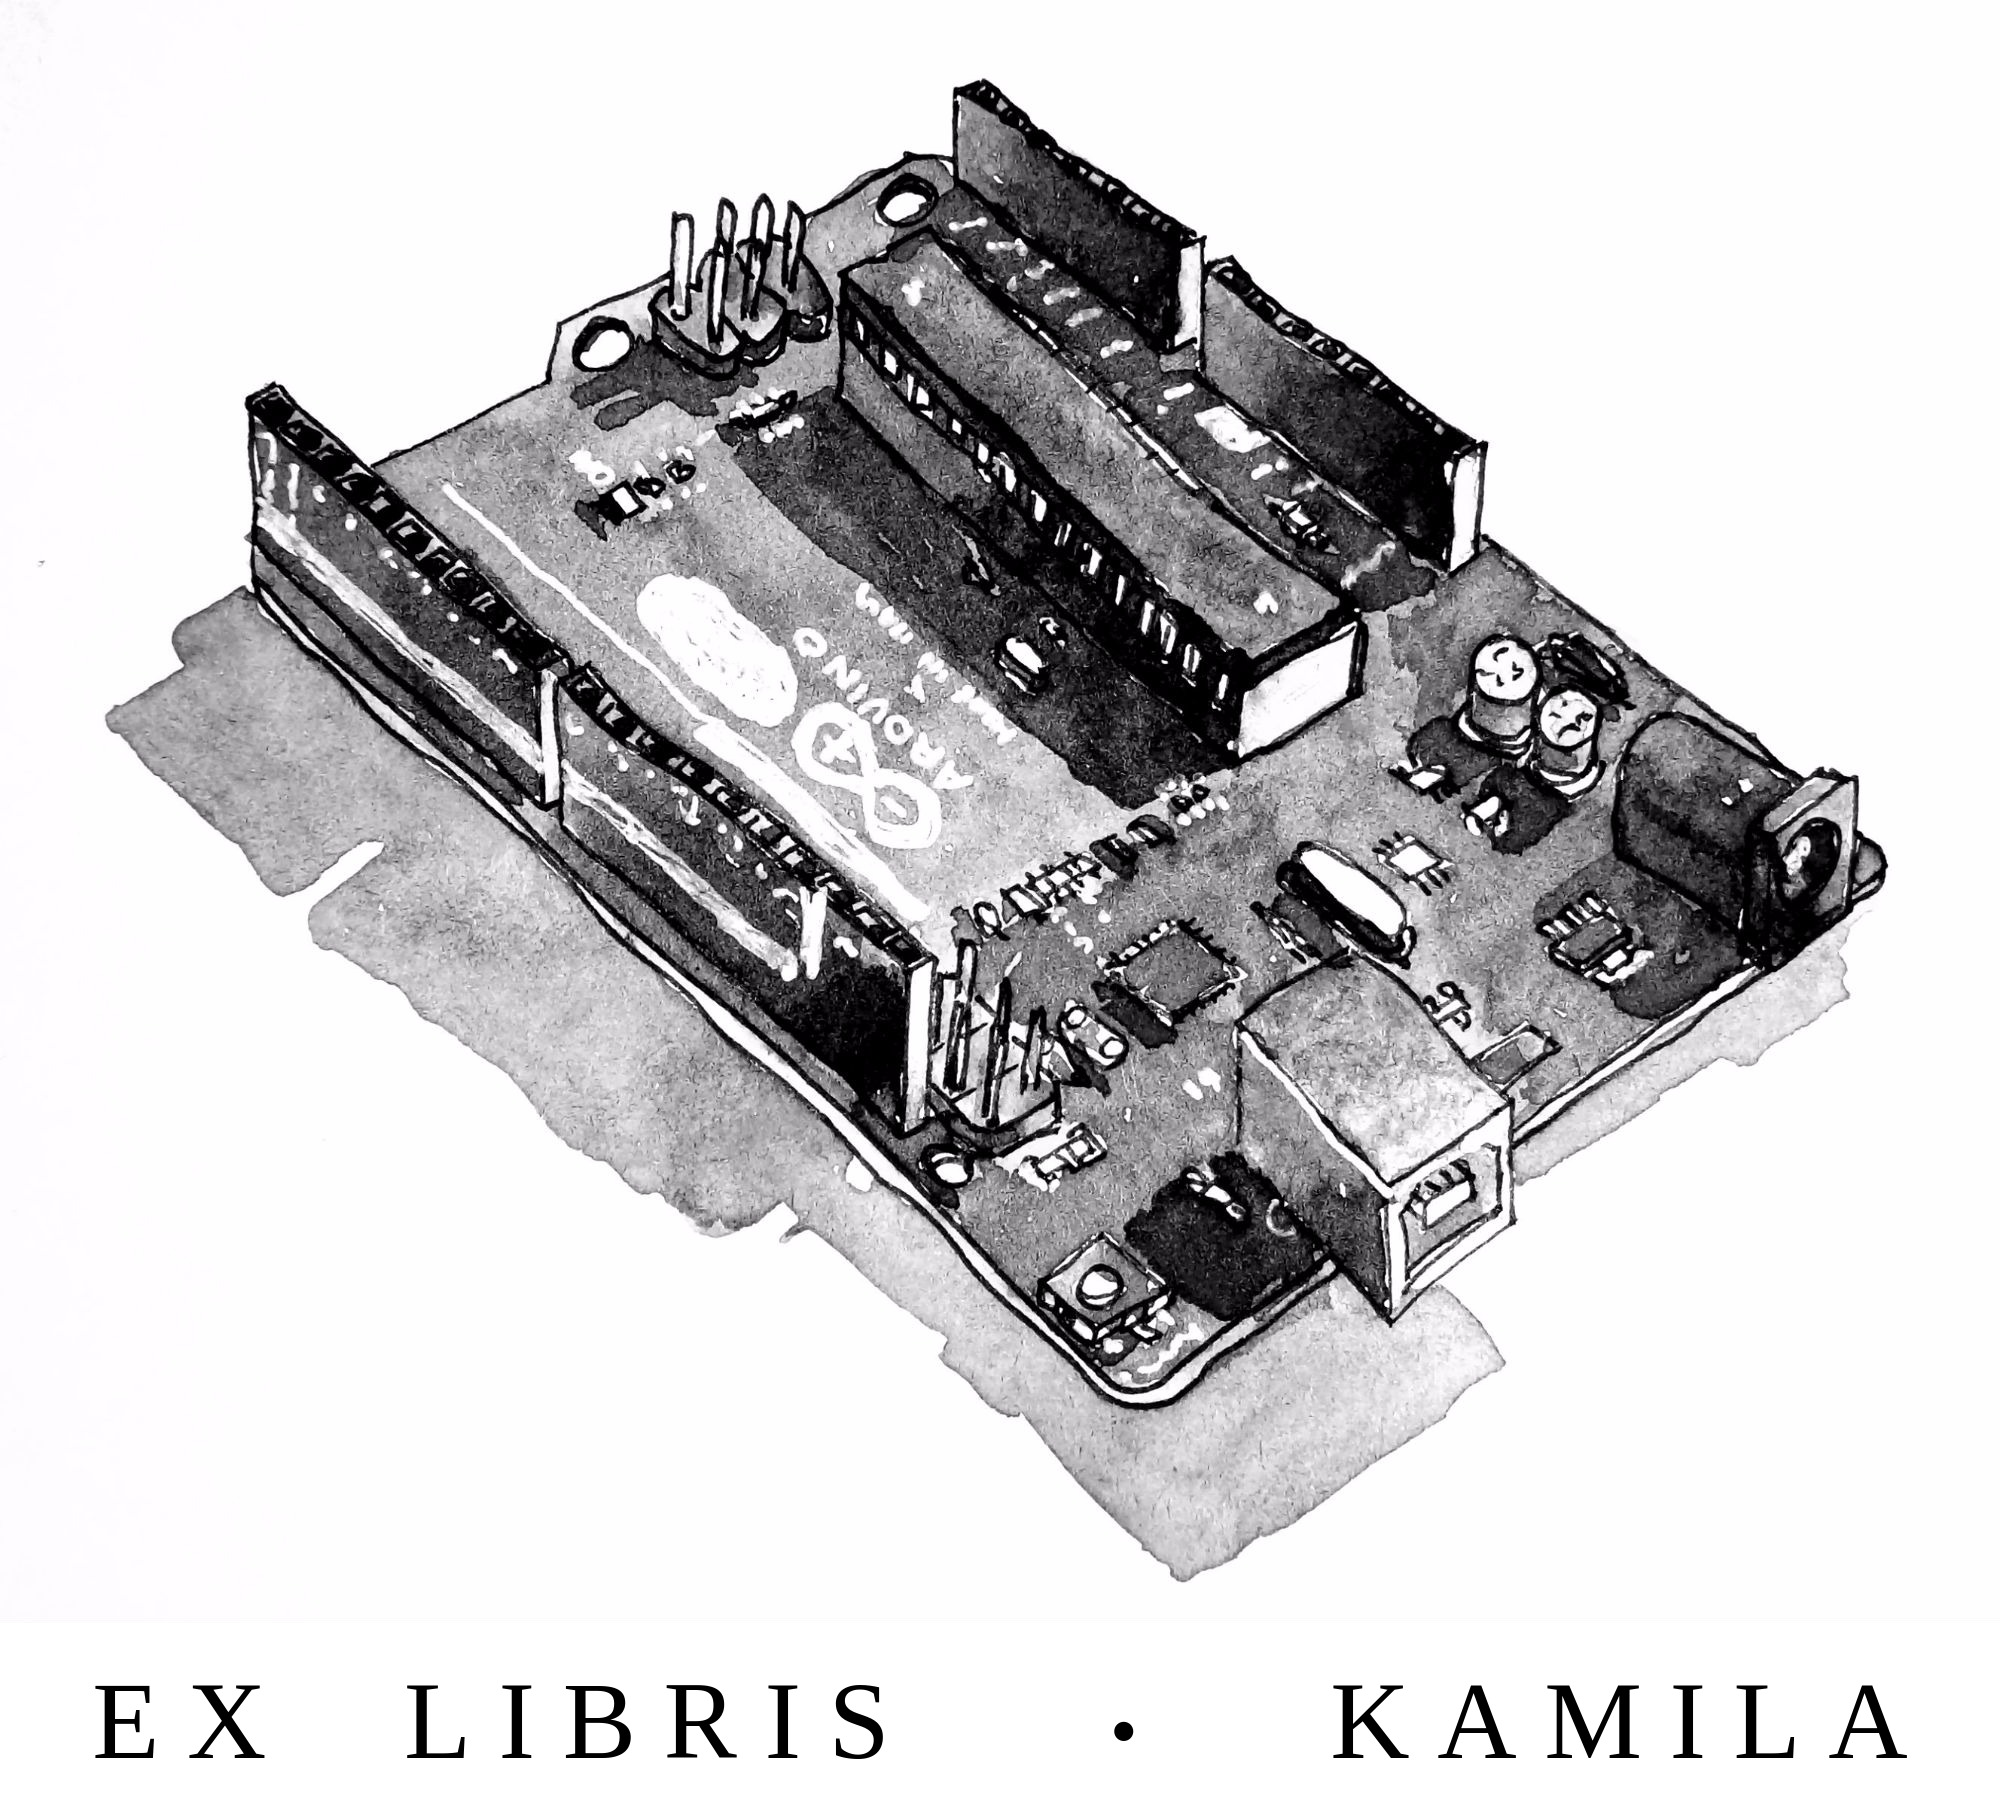
\includegraphics[width = 80mm]{arduino_dwg.jpg}

\vspace*{2cm}

Copyright \textcopyright \, J. Aleksanderek, K. Zdybał, 2017

For more projects similar to this one

visit me on GitHub: @camillejr

To contact me personally drop me a line at:

\verb|kamilazdybal@gmail.com|


\vspace*{2cm}

\verb|Objectif Morse|

\verb|version 1.0|
\end{center}
\newpage




\setlength{\parindent}{0cm}
\clearpage

\tableofcontents

\setlength{\parskip}{1em}
\renewcommand{\baselinestretch}{1.0}

\chapter{Introduction}\label{chap:intro}

\textbf{Welcome to the \textit{Objectif Morse} project.}

You will soon begin a journey through secret coded messages transmitted between powerful computers over tiny distances.

The first purpose of this document is to keep the record of the work that we did, the ideas and the solutions that we came up with and of the things that we have learned.

The second and more important purpose is to serve as a tutorial for you, if you ever feel like embarking on the same adventure as we did. Following the document you should be able to accomplish the same mission and maybe even extend it with your own ideas. This journey will increase your knowledge in C++, Linux, Arduino, electronics and, undoubtedly, French language. Either some basic understanding in all of these is required as a prerequisite, or a strong will to invest time and effort to learn many new things as you go.

This project is aimed for explorers and experimenters for whom it may seem difficult at first. But we believe that the spirit of "learning by doing" is the most effective way to understand the difficult. 

All the codes produced are not included in this document. You can download everything needed from our \href{https://github.com/camillejr/objectif_morse}{GitHub repository}.

Reach out to section \ref{sec:equip} to check if you have everything that you will need!

It's time to present the mission objectives...

\section{Voici l'Objectif Morse}

You type a secret message on a stationary computer into the terminal. This message is translated into Morse alphabet and the signal of dots and dashes is sent to the parallel port as high and low states. The parallel port pins are connected to a small circuit with an LED diode, which blinks accordingly to the message translation. No spies should be observing the diode. This message is received by a phototransistor, situated in the close proximity of the LED. The phototransistor passes the signal to the Arduino device. Arduino connected to a portable computer prints the received message in Morse on the Serial Monitor. The message is translated to regular text after reading the Arduino output and printed in the terminal of the portable computer. 

The message is received and the war is won.

\subsection{Choice for the project name}

The idea for this project was born while reading \textit{Les Aventures De Tintin}, comic books written by a belgian cartoonist Hergé, where messages transmitted in the Morse code are a common form of communication. 

The name \textit{Objectif Morse} is a reference to one of our favourite books in the series \textit{Objectif Lune} \cite{objectif_lune} (eng. \textit{Destination Moon}), and is hence a tribute to our initial inspiration.

\begin{figure}[H]
\centering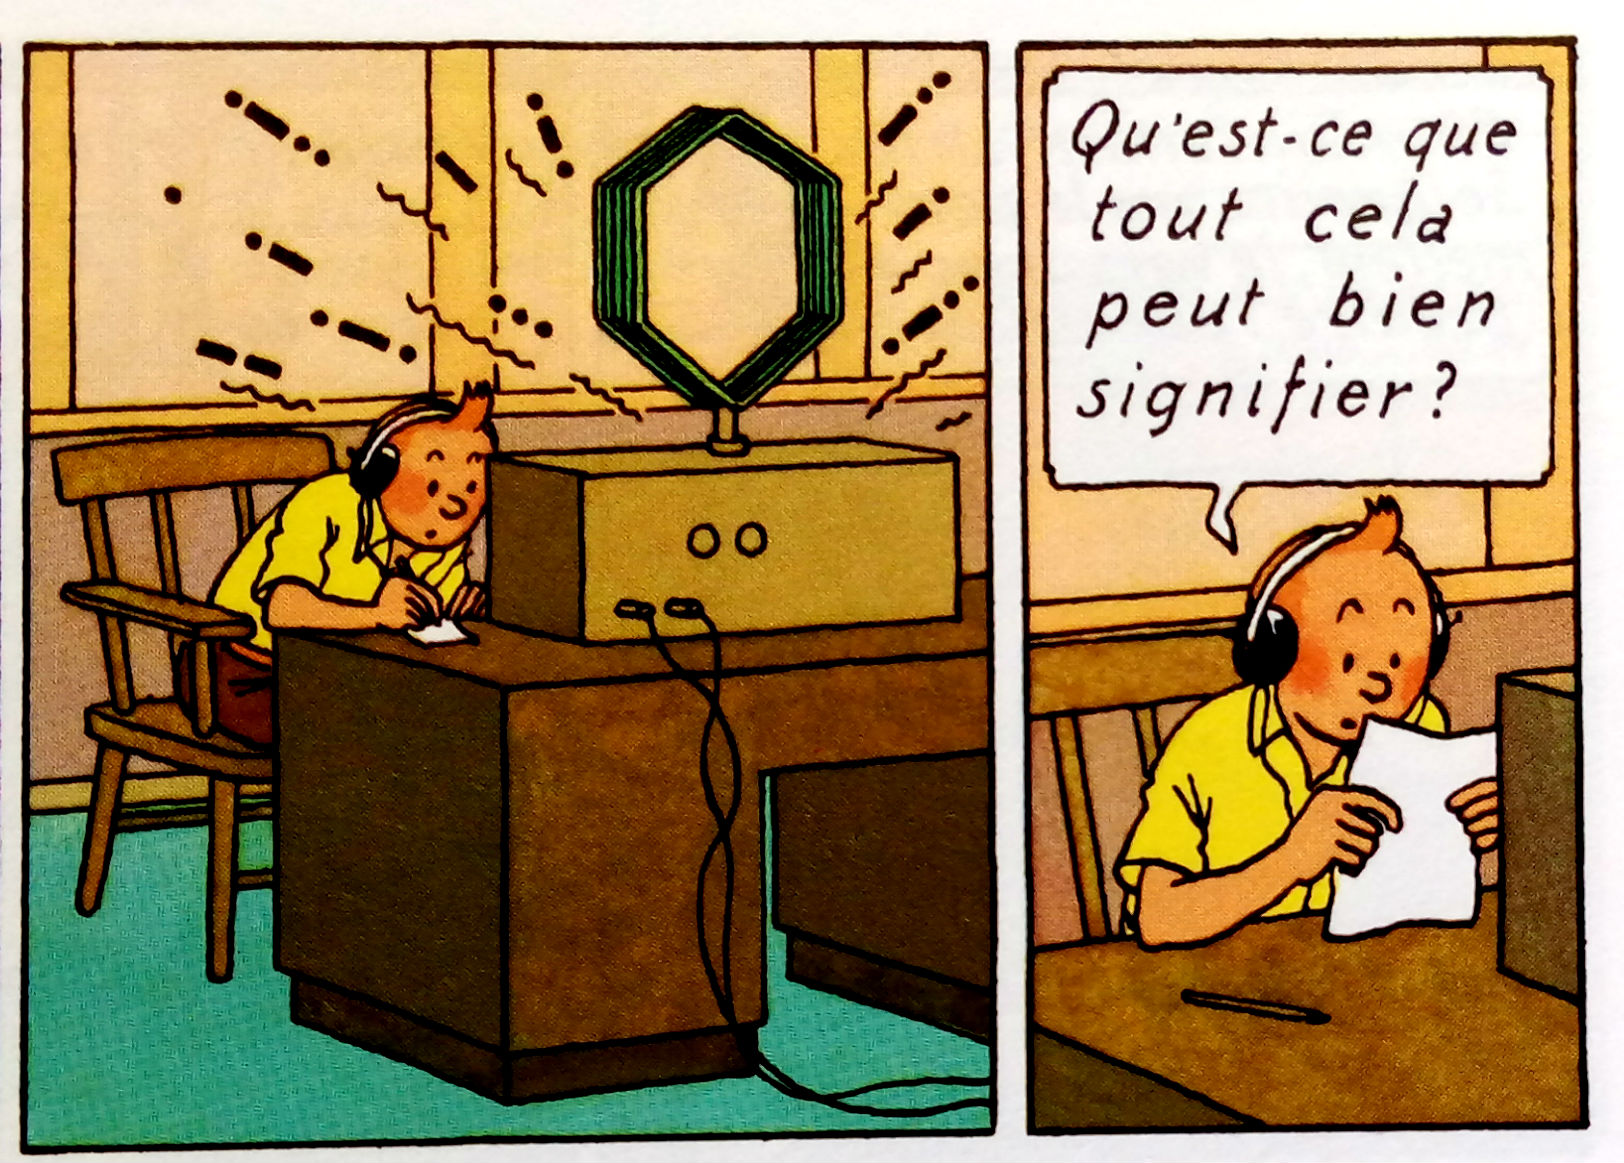
\includegraphics[scale=0.1]{le_lotus_bleu}
\caption{Excerpt from \textit{Les Aventures de Tintin: Le Lotus Bleu} by Hergé \cite{le_lotus_bleu}}			
\label{fig:tintin}
\end{figure}

\section{Preparation} \label{sec:equip}

\subsection{Project phases}

This project is divided into two phases: \textbf{broadcasting} and \textbf{receiving}. 

These two phases don't require each other to get them working, however, the \textbf{receiving} phase needs a light trigger to obtain a signal. If you didn't build the  \textbf{broadcasting} phase, you can use for example the light from a flashlight. Nevertheless, it's not recommended from the debugging point of view, unless you are an expert in broadcasting Morse signals by hand.

The two phases are separated by a few centimetres air gap. What happens inside of the air gap shall remain a secret.

\subsection{Equipment used} 

Electronics:

\begin{enumerate}

\item LED diode
\item phototransistor
\item resistors: 330 Ohm, 10 000 Ohm
\item a few cables
\item at least one breadboard but best to have two
\item parallel port plug with soldered cables

\end{enumerate}

Computation:

\begin{enumerate}

\item Arduino Uno with a USB A-B cable
\item stationary computer with Linux
\item portable computer with Linux
\item of course you need some monitors and keyboards...

\end{enumerate}

Optional:

\begin{enumerate}

\item flashlight - increases the interactivity of this project

\end{enumerate}

\newpage

\subsection{Code used}

The \textit{Objectif Morse} project is coded in C++ language.

This is a scheme of how the code should be distributed over devices:

\textbf{Stationary computer}

\begin{verbatim}
	broadcastMain.cpp
	morse.cpp
	morse.h
	sendToPort.cpp
	sendToPort.h
	makeFileB
\end{verbatim}

\textbf{Portable computer}

\begin{verbatim}
	arduinoReceive.cpp
	arduinoReceive.h
	receiveMain.cpp
	makeFileR
\end{verbatim}

\textbf{Arduino}

\begin{verbatim}
arduinoCode.ino
\end{verbatim}

In order to download our GitHub repository with all the necessary codes it's best to have \verb|git| installed on your computers. Then type in the command line:

\begin{snugshade}
\verb|git clone https://github.com/camillejr/objectif_morse.git|
\end{snugshade}




\section{Morse alphabet}

The Morse alphabet characters are the following:








The Morse alphabet is scalable, which means that you can set the \verb|dotTime| to whatever time you need, and all the remaining intervals will simply become a corresponding multiple of that unit.


\section{Legal note}

First, it is possible that things won't work when you put the cables together. Second, it is possible that the code we produced contains bugs and might cause unexpected behaviours. Third, it is possible that certain favourable conditions\footnote{it is quite common among computers that the nerby presence of certain objects, or certain position with respect to certain constellations, or certain mysterious words in certain forgotten config files is causing things to work.} arised when we were working on this project and it might take some effort to make them reappear again.

If you have just said: \textit{"How awesome! I can't wait do deal with that!"}, then you're the right person in the right place. We wish you a lot of errors as you go, because you're going to learn a lot from them. 

\newpage

\chapter{Broadcasting}

\verb|OBJECTIF_MORSE, PHASE: BROADCASTING -| the first phase of the \textit{Objectif Morse} project is to translate the secret message from the regular text to the Morse alphabet. This part comprises the message input using alphanumeric characters into the terminal where the broadcasting code is running. The message is translated by the program and broadcasted on an LED diode connected to the parallel port output pin.

\section{Code description}

The code for broadcasting the secret message in Morse consists of 5 files plus a makefile.

The code is split into user input/output interactive part (\verb|broadcastMain.cpp|), into functions that operate on messages (\verb|morse.cpp| and \verb|morse.h|) and into sending output to the parallel port (\verb|sendToPort.cpp| and \verb|sendToPort.h|).

The most important constituents of each file are presented in the graph below:

\begin{figure}[H]
\centering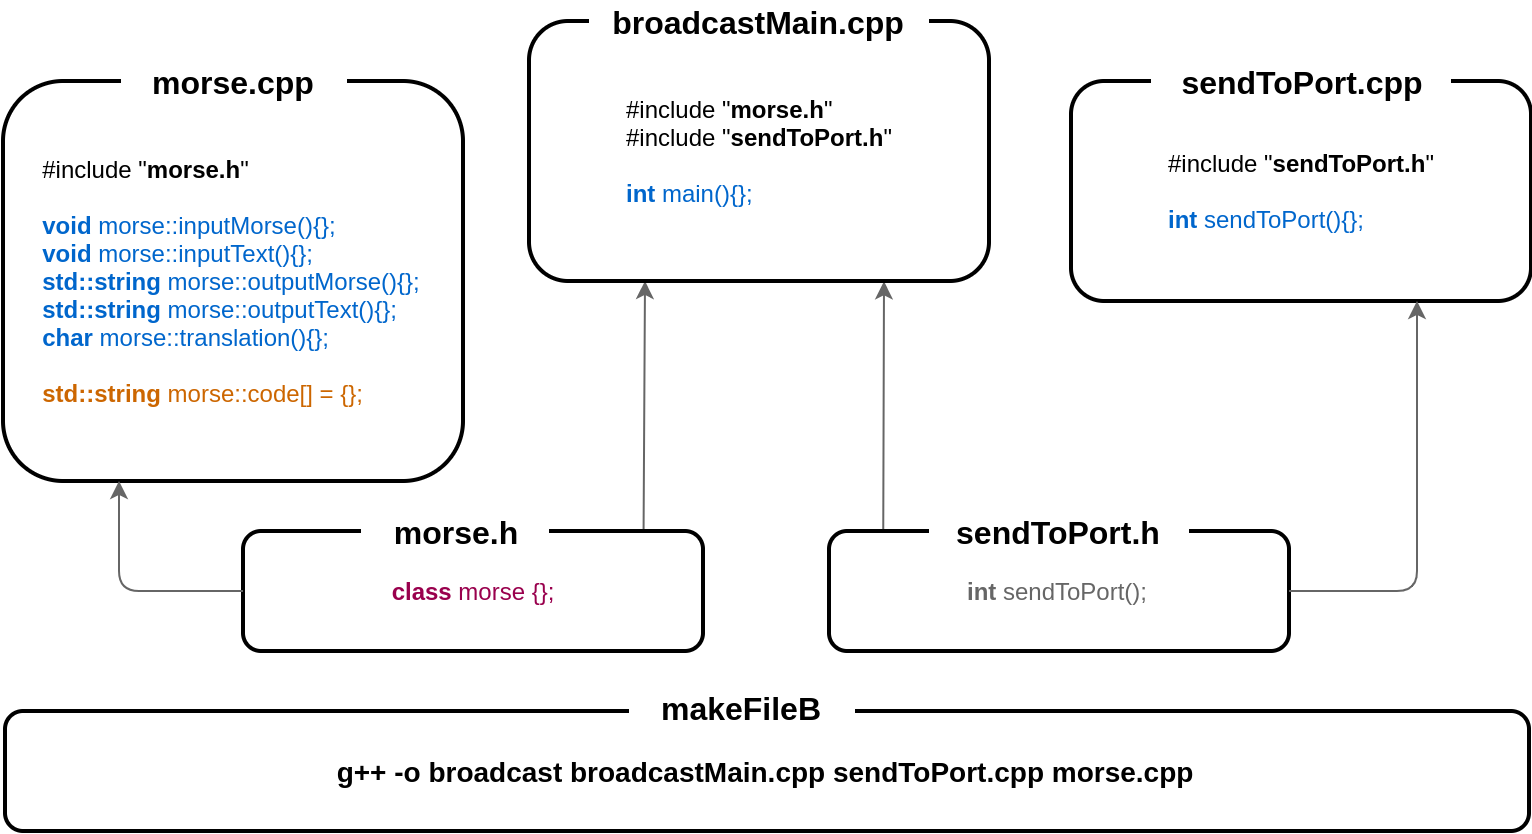
\includegraphics[width=15cm]{bCodeStructure}
\caption{Code structure for the \textbf{broadcasting} phase.}				
\label{fig:br_code}
\end{figure}

\subsection{Class \texttt{morse}}

We created a class called \verb|morse| that handles all the necessary variables and functions corresponding to translating from \verb|text > morse| and from \verb|morse > text|.

The definition of the class is presented in the listing below:

\begin{lstlisting}
class morse
{

	public:
	void inputMorse(std::string);
	void inputText(std::string);
	std::string outputMorse();
	std::string outputText();

	private:
	std::string morseMessage;
	std::string textMessage;
	static std::string code[];
	char translation(std::string);

};
\end{lstlisting}

\subsection{Functions and variables}

In this subsection we are going to take a closer look into what the functions and variables declared inside the \verb|morse| class do. This part is for you to get a quick overview and to help you glue the things together in your head before you read the section \ref{sec:howB}, which describes the inner cogs much deeper.

\textbf{Functions}

\verb|morse::inputMorse()| - takes a string written in Morse alphabet as an input. Ideally, the input string should only consist of the following characters:

\begin{enumerate}
\item dot \verb|"."|

\item dash \verb|"-"|

\item space \verb|" "|

\item slash \verb|"/"|
\end{enumerate}

If the user inputs characters other then the listed above, they will be treated as unknowns in the message.

\verb|morse::inputText()| - takes a string written in alphanumeric alphabet as an input. The input string should only consist of:

\begin{enumerate}
\item letters \verb|A-Z| (\verb|a-z|)
\item numbers \verb|0-9|
\item space \verb|" "|
\item full stop \verb|"."|
\item comma \verb|","|
\end{enumerate}

If the user inputs characters other then the listed above, they will be ignored in the message.

\verb|morse::outputMorse()| - function that returns the ready string consisting of message written in Morse alphabet.

\verb|morse::outputText()| - function that returns the ready string consisting of the message written in alphanumeric characters.

\verb|morse::translation()| - translates a series of dots and dashes from the Morse message to the ASCII sequence.

\textbf{Variables}

\verb|morse::morseMessage| - contains message written in the Morse alphabet.

\verb|morse::textMessage| - contains message written in the alphanumeric characters.

\verb|morse::code| - an array of strings that create the Morse alphabet table. A closer description of this array is given in section [\ref{sec:asciitomorse}].


\subsection{Main}

The "Main" of the broadcasting phase is included in the file \verb|broadcastMain.cpp|. This is where a lot of messing around can be performed, because this code is just calling our already preciously prepared pieces. If you don't like our implementation of the user interface in the \textit{Objectif Morse} project, you have a lot of freedom to play with this file.

There is one interesting behaviour that can be controlled from the \verb|main| function - speed of the transmission, or more precisely - the duration of one "dot" signal in the Morse alphabet. This duration in micro seconds is initially set to 25000 (0.25 second) when calling \verb|sendToPort| function: 

\begin{lstlisting}
sendToPort(secretMessage.outputMorse(), 1, 25000);
\end{lstlisting}

but can be adjusted to your needs.

\subsection{Fire it up with makefile}

To compile the code on your computer you can use the makefile \verb|makeFileB|.

Simply teleport yourself to the place where the 5 files are placed and at that location run from the command line:

\begin{snugshade}
\verb|make -f makeFileB|
\end{snugshade}

This will result in the creation of one more file, a binary called \verb|broadcast|.

To fire up the whole code structure (in fact, to primarily run the \verb|main| function from \verb|broadcastMain.cpp|) type in the command line:

\begin{snugshade}
\verb|./broadcast|
\end{snugshade}


In certain cases you may need to run the binary as \verb|root|:

\begin{snugshade}
\verb|sudo ./broadcast|
\end{snugshade}

and type in your root password.

\subsection{Test run}

One thing that you can do right now is to ask the program to translate something for you! After the code is started you should see:

\begin{snugshade}
\begin{verbatim}
Select translation:
1) Text to Morse
2) Morse to text
\end{verbatim}
\end{snugshade}

Type either 1 or 2 to select an option and then input the message to translate it!

As long as the electronics isn't connected to the parallel port, when you select 1, nothing more spectacular should happen.

Any errors in trying to send the message to the parallel port will result in an error message at the end of the translation:

\begin{snugshade}
\begin{verbatim}
Select translation:
1) Text to Morse
2) Morse to text
1
Type text message:
Hello world
You've typed: 
Hello world
Morse code: 
.... . .-.. .-.. ---   .-- --- .-. .-.. -.. 
Error sending message to parallel port.
\end{verbatim}
\end{snugshade}

The functionality to translate from Morse to text has been added mostly for fun here. When you input message directly in Morse alphabet it won't be transmitted, this is because our initial objective was to input secret message in regular text. Feel free to translate the subtitle from the front page of this document!

\section{How does it work} \label{sec:howB}

This section is diving a little deeper into explanation of the ideas behind the \textbf{broadcasting} phase. It also tells you how to set up the electronics part and hence we hope that things will get much more fun right now!

\subsection{Parallel port connection}

In this section we describe how to connect to the parallel port (parport\footnote{if you wish to sound more technical.}) and how to build a simple circuit with an LED diode. Notice that not every computer has got a parallel port. Usually, a portable computer will not be equiped with a parport, so try to get one oldschool stationary computer like we did! The parallel port is big and pink like this one:

\begin{figure}[H]
\centering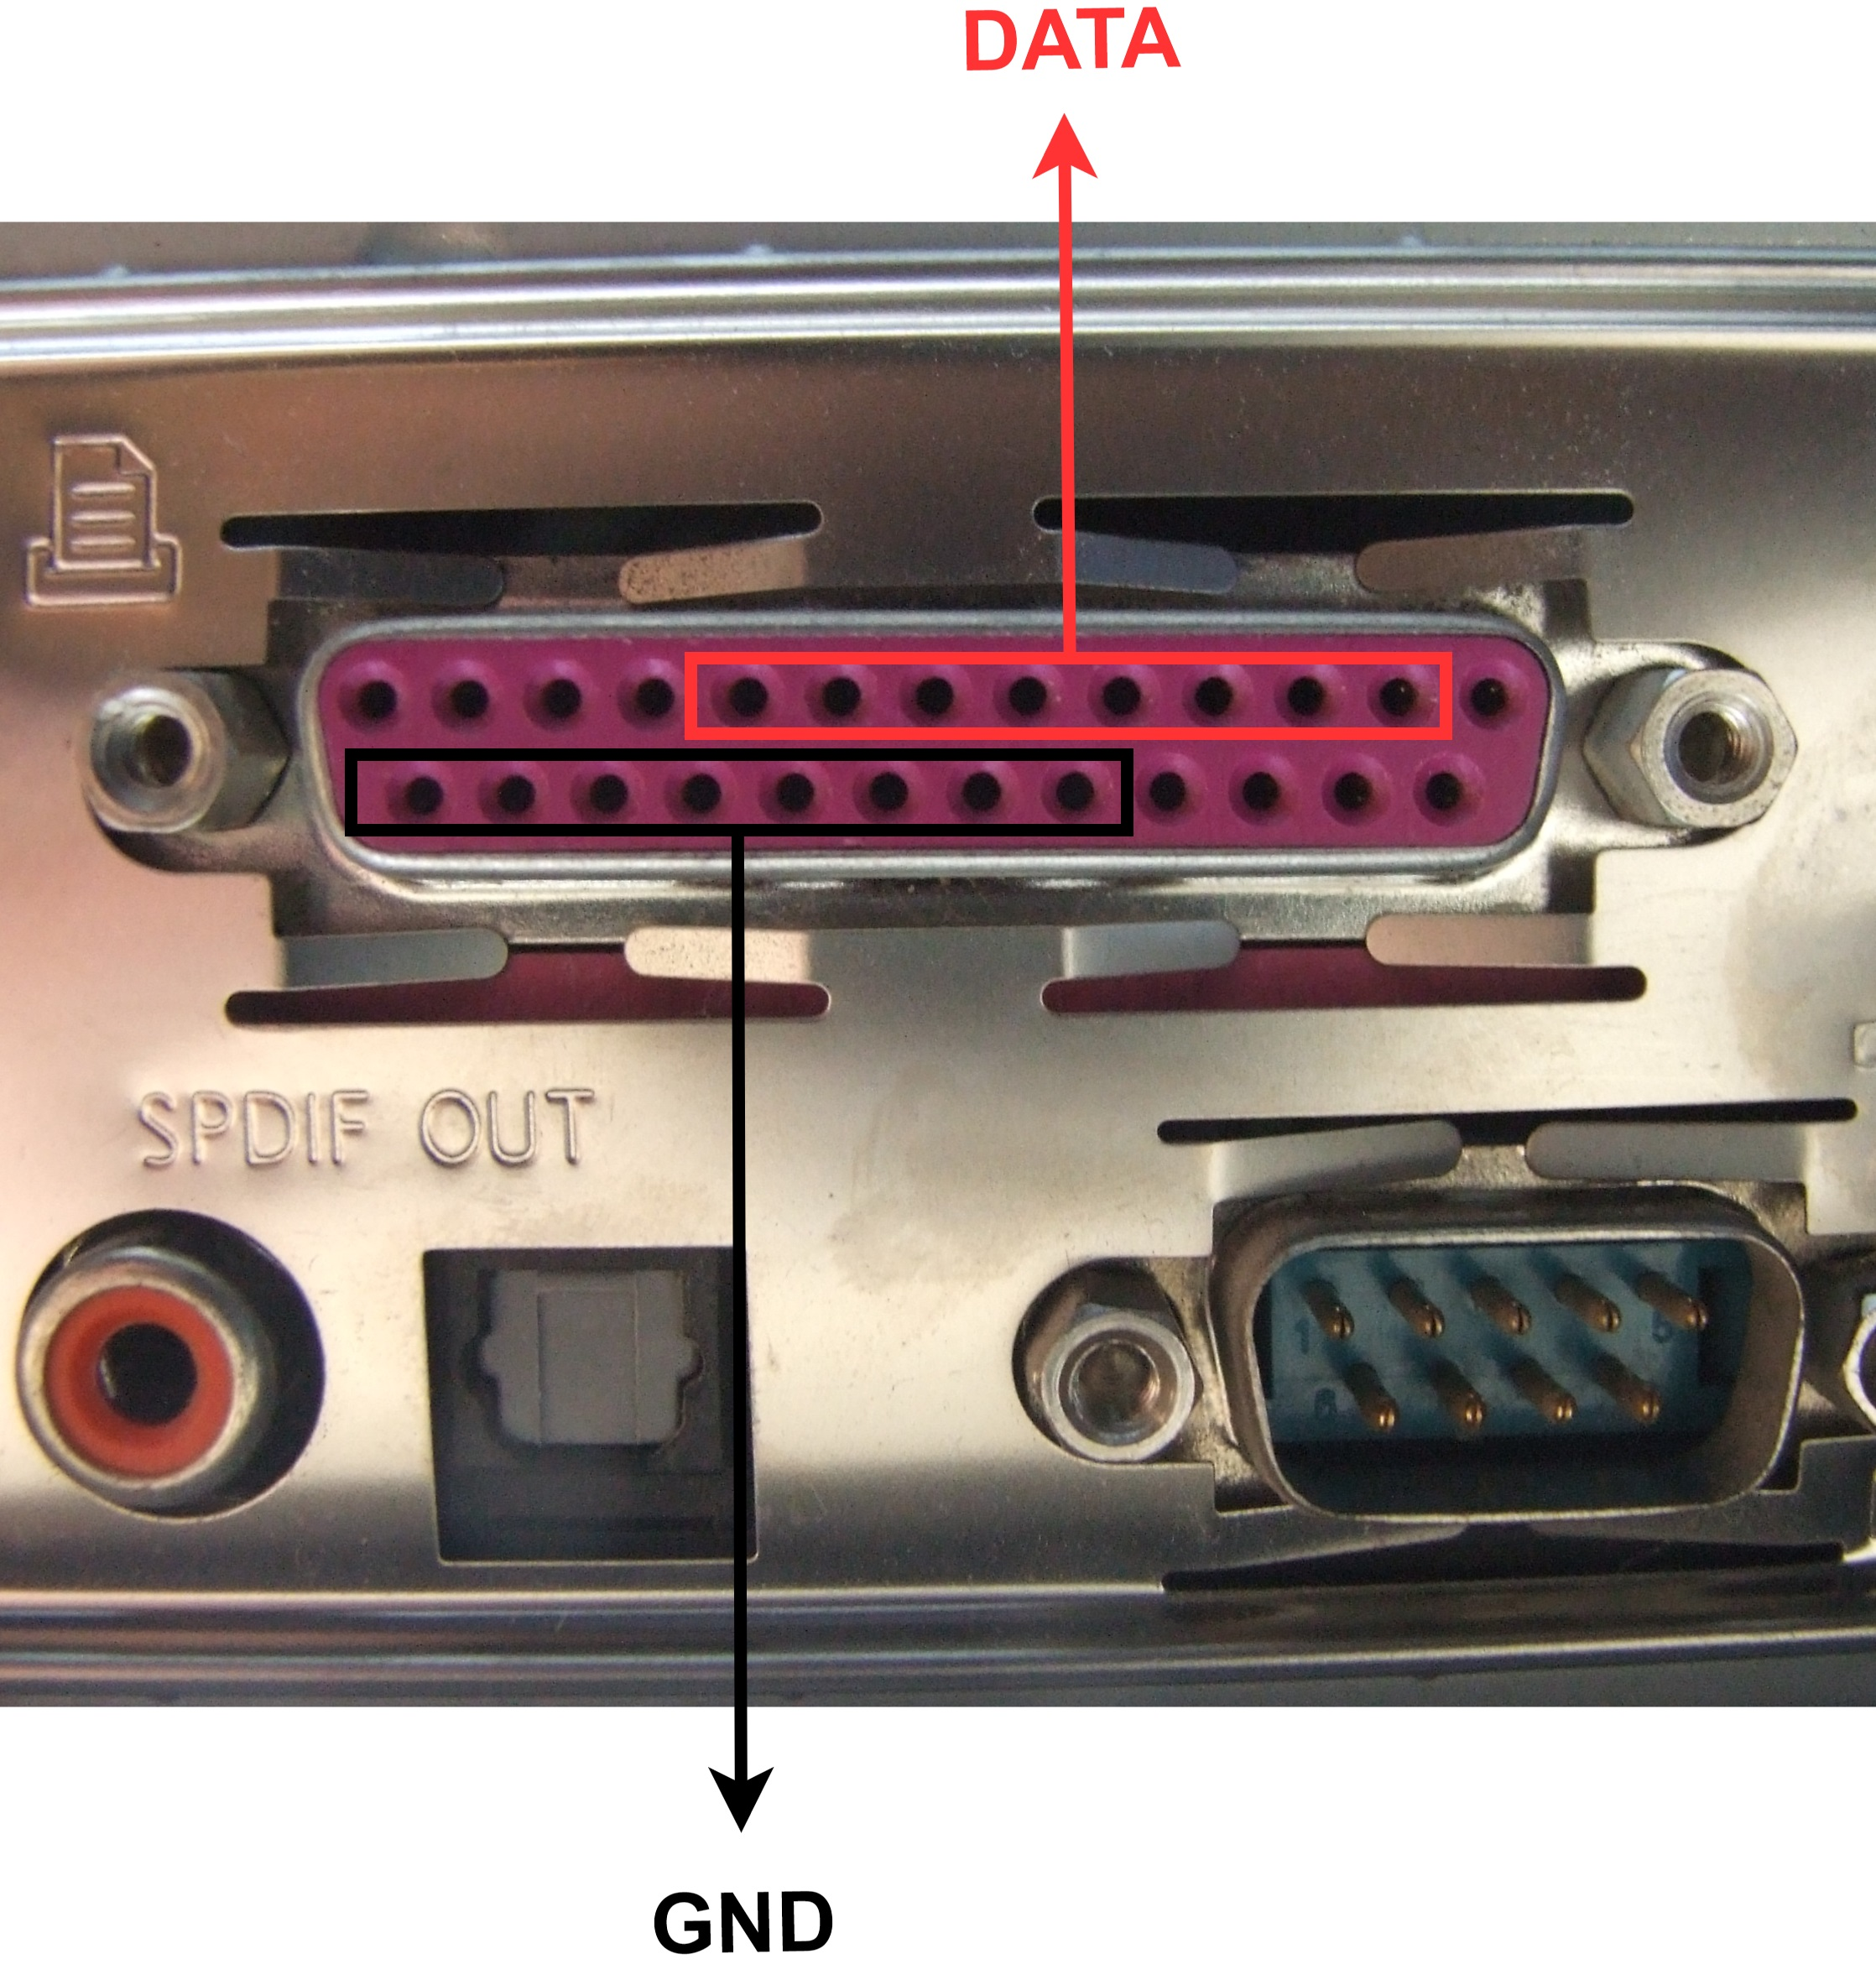
\includegraphics[width=8cm]{par_port}
\caption{Parallel port pins: DATA and GND.}				
\label{fig:par_port}
\end{figure}

You should be mostly interested in two sets of pins here - data pins (DATA) and ground pins (GND). There's eight data pins, marked in red in the picture above. They will serve as our (+) and they are the ones, who's high and low states can be controlled from the program. There's also eight ground pins, marked in black in the picture and they serve as our (-).

It doesn't really matter which ground pin you connect to. It also doesn't matter which data pin you connect to but you should adjust the value in the place of \verb|yourNumber| in the file \verb|sendToPort.cpp|:

\begin{snugshade}
\verb|ioperm(base, yourNumber, 1)|
\end{snugshade}

By this value you specify up to which DATA pin you give the permission to connect to. For example, if you set \verb|yourNumber = 3|, you will be allowed to use pins: first, second and third. Since we only needed one DATA pin to connect to, we've given ourselves permission to access just the first one, so this value is 1 by default. To read more about \verb|ioperm| check out this page \cite{ioperm}.

You should also be equipped with a parallel port plug. The best idea is to solder ground and data cables so that they stick firmly to the plug. Here's the picture of our plug, connected to the cables:

\begin{figure}[H]
\centering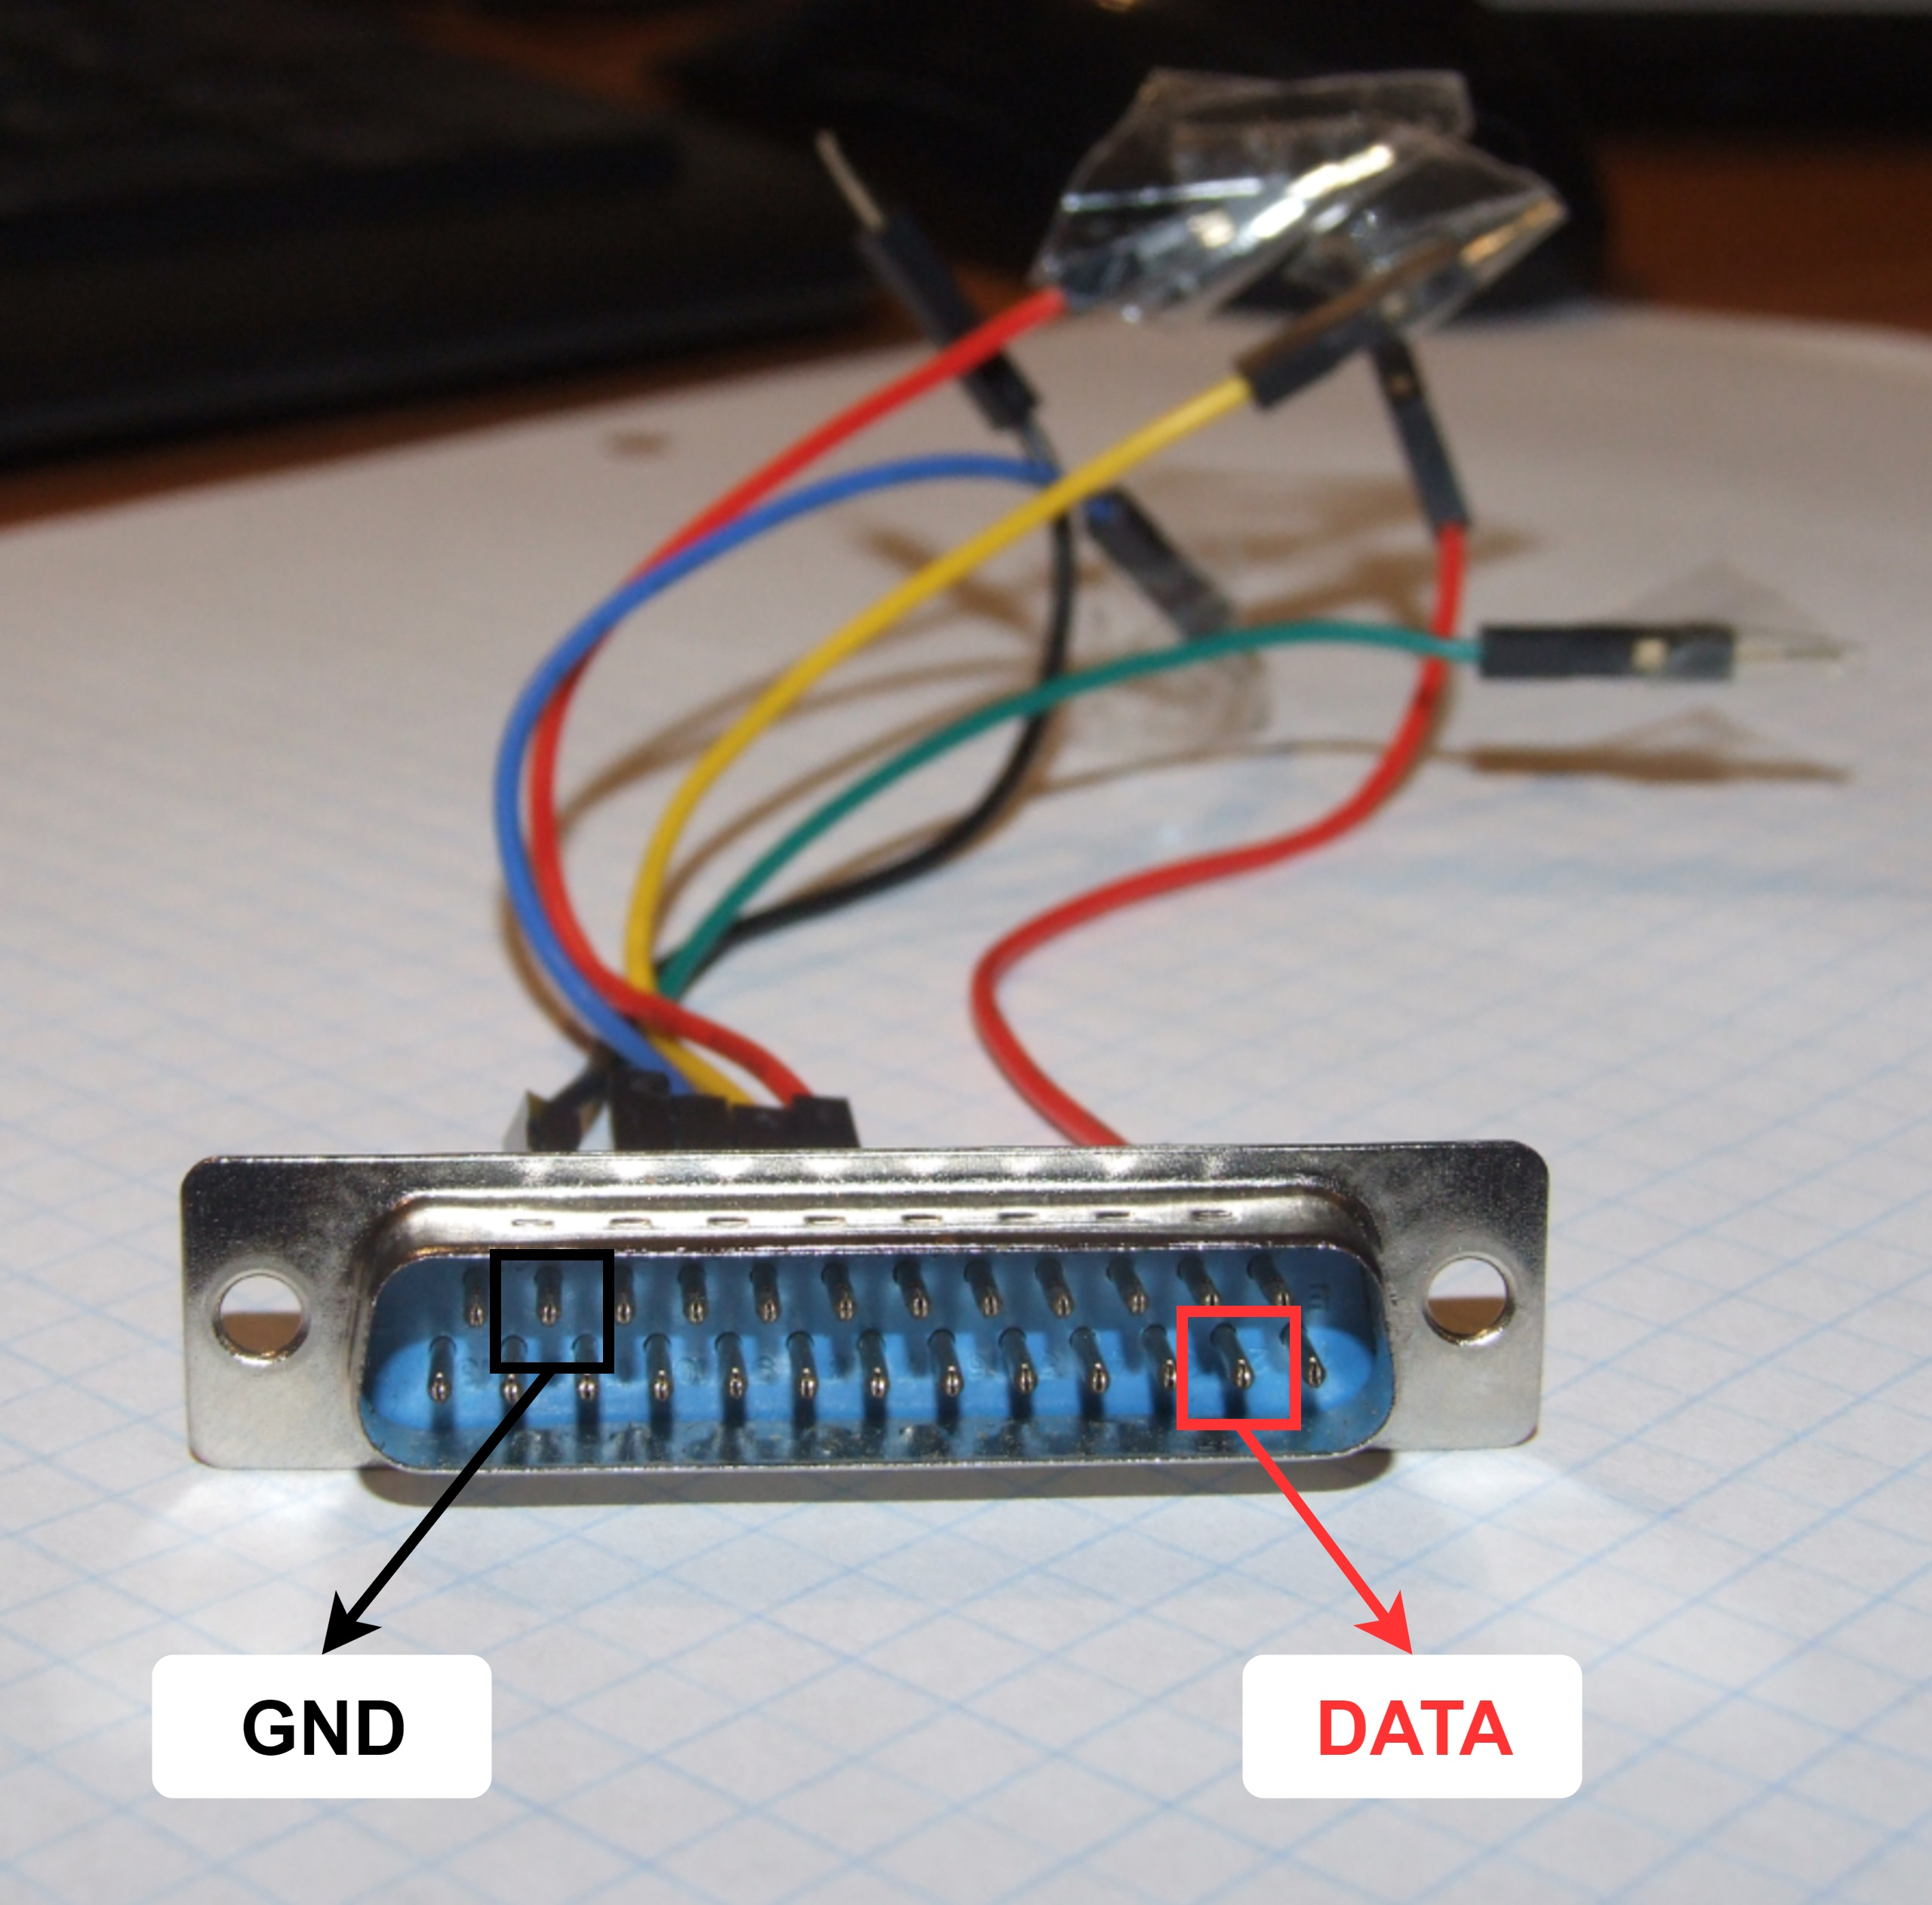
\includegraphics[width=8cm]{parport_plug}
\caption{Parallel port plug.}				
\label{fig:parport_plug}
\end{figure}

Remember that you only need two cables - one ground and one data. You don't have to worry about other colourful cables in the picture above.

The final thing to do is to build the rest of the circuit connected to the plug, which is very simple! It only consist of an LED diode and a 330$\Omega$ resistor.

\begin{figure}[H]
\centering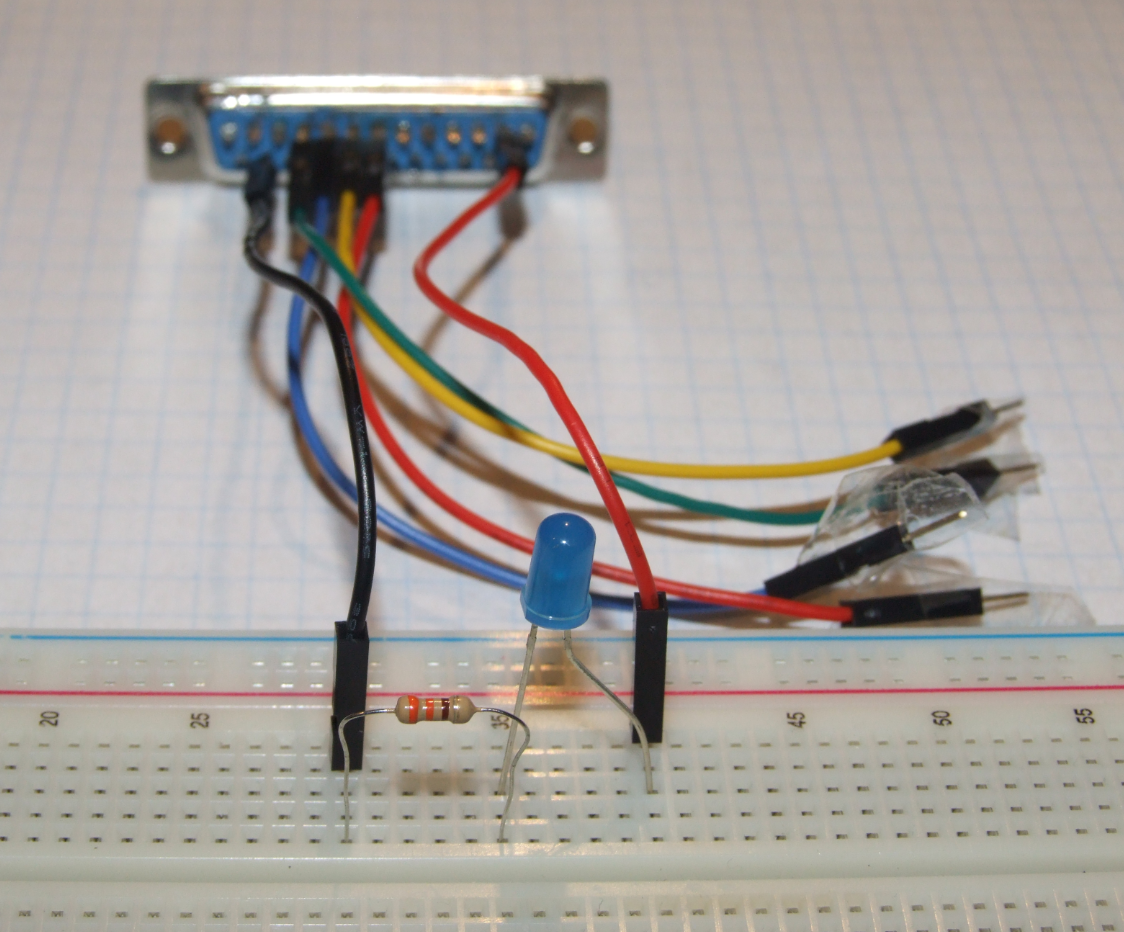
\includegraphics[width=8cm]{broadcast_circuit}
\caption{Electronic circuit for broadcasting.}				
\label{fig:broadcast_circuit}
\end{figure}

\subsection{Alphanumeric to Morse} \label{sec:asciitomorse}

Probably the most important (and interesting) part of the \textit{Objectif Morse} is the introduction of the Morse alphabet in the code. Each letter \verb|A-Z| (\verb|a-z|) and each digit \verb|0-9| has got its representation in the Morse alphabet. Notice also, that the Morse alphabet is not case sensitive and both lower-case and upper-case letters translate to the same Morse character. So how can the sequence of dots and dashes be implemented in C++?

The definition of the Morse alphabet is present in the file \verb|morse.cpp| inside the variable called \verb|morse::code|. This is an array of strings that contains all Morse alphabet characters. Its graphical representation is shown below:

\begin{figure}[H]
\centering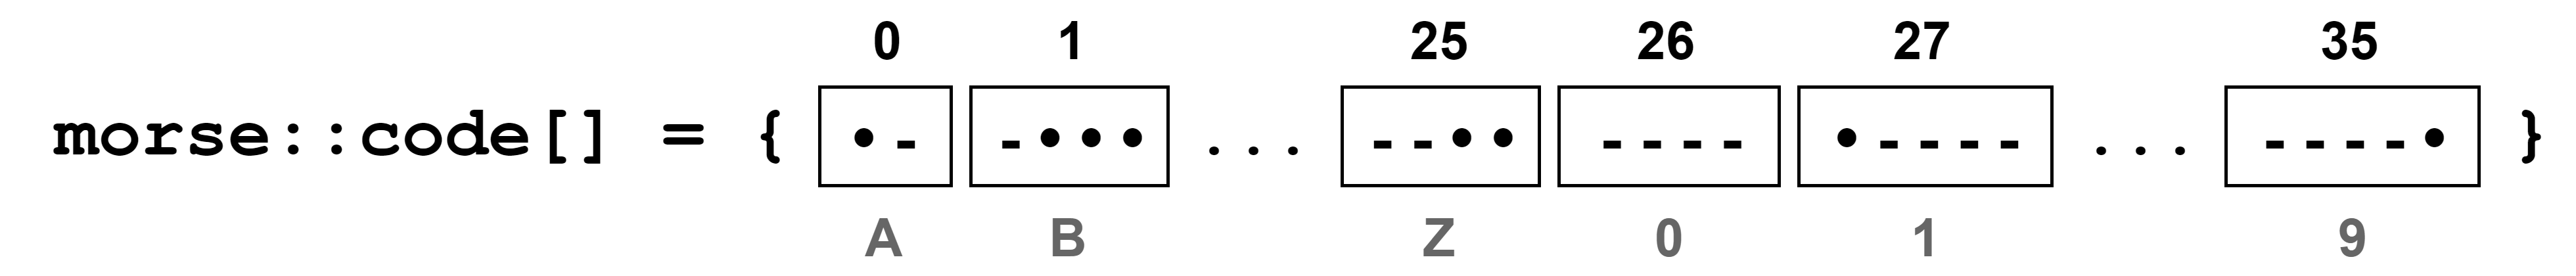
\includegraphics[scale=0.1]{morse--code}
\caption{Morse code array.}				
\label{fig:morse_code_array}
\end{figure}

Every ASCII character is assigned a number, which inside the C++ language can be retrieved by casting the character into an integer. This is done by the following line inside the function \verb|morse::inputText()|: 

\begin{lstlisting}
num = (int)textMessage[n];
\end{lstlisting}

For example, for a \verb|textMessage| character equal to "\verb|f|" the parameter \verb|num| will be equal to 102.

For the characters used in this project we have the following ASCII numerations:


\begin{enumerate}

\item upper-case letters \verb|A-Z| : 65 - 90

\item lower-case letters \verb|a-z| : 97 - 122

\item digits \verb|0-9| : 48 - 57

\item space \verb|" "| : 32

\item full stop \verb|"."| : 46

\item comma \verb|","| : 44

\end{enumerate}


We have then decided to map every legal alphanumeric ASCII character into the created array. This means that each alphanumeric character number gets the number of its position inside the \verb|morse::code| array. This is achieved by subtracting certain number from the ASCII numeration. The graphical representation of this mapping is presented below:

\begin{figure}[H]
\centering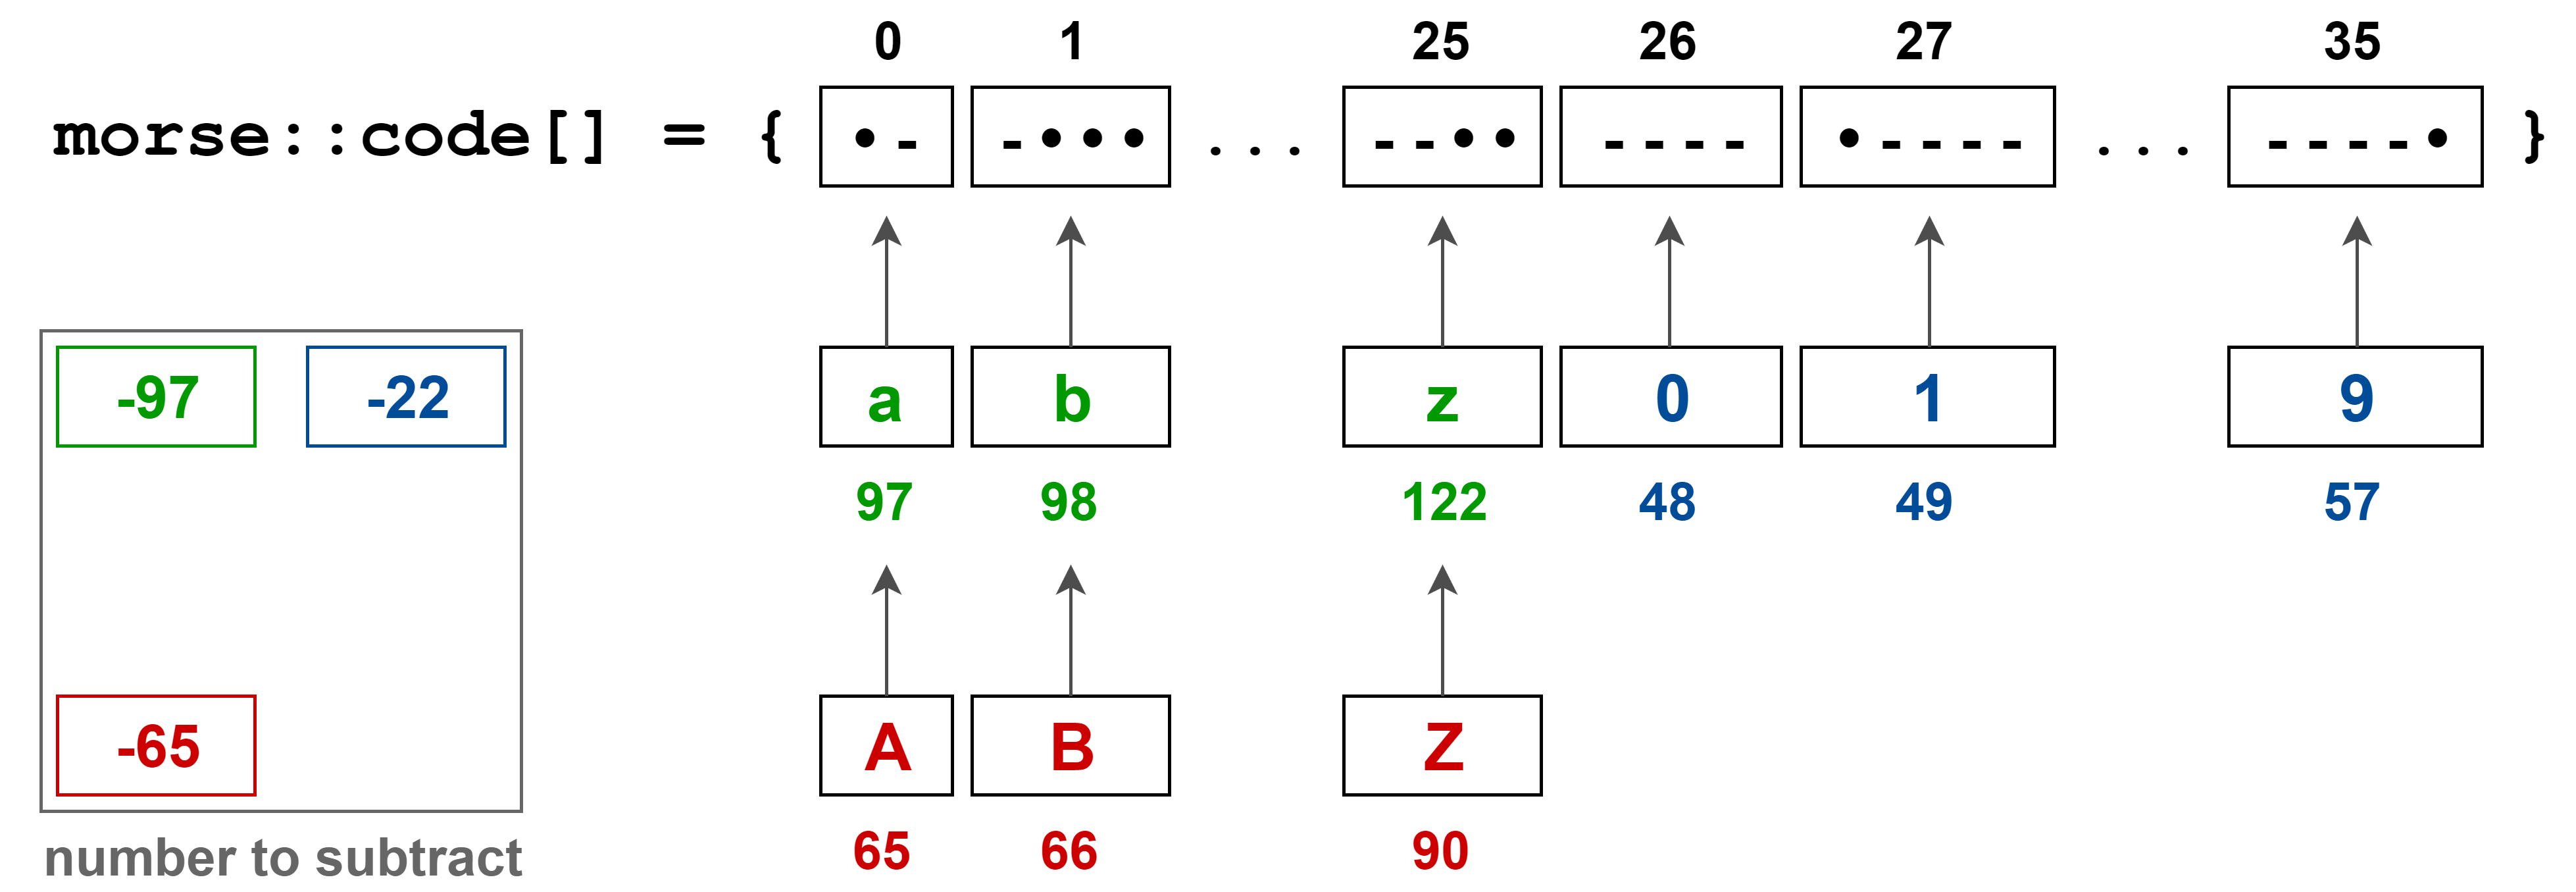
\includegraphics[scale=0.1]{morse_code_map}
\caption{Mapping alphanumeric characters to the morse code array elements.}				
\label{fig:morse_code_map}
\end{figure}

Inside the code we have therefore:

\begin{lstlisting}
if (num > 64 && num < 91) morseMessage += code[num - 65];
	else if (num > 47 && num < 58) morseMessage += code[num - 22];
	else if (num > 96 && num < 123) morseMessage += code[num - 97];
\end{lstlisting}

Using our previous example, the character "\verb|f|" will result in \verb|num| = 102 and since this number is between 96 and 123 (lower-case character), the number subtracted will be 97. This will altogether result in the position with index 5 in the \verb|morse::code| array, which corresponds to a string "$\cdot\cdot$\text{-}$\cdot$". 

This string will be added (\verb|+=|) to the message translation variable \verb|morseMessage|.

With each run of the \verb|for| loop in the \verb|morse::inputText()| function, the coded message will be appended by the next Morse code character.

Notice that there is also an \verb|else| statement, which takes care of other non-alphanumeric characters which the user can type. The legal non-alphanumeric characters includes a full stop, a space and a comma. Every other character is by default replaced with a space in the translation.


\begin{lstlisting}
else
{
  switch (num)
  {
    case 46:
    {
      morseMessage += "/";
      break;
    }
    case 32:
    {
      morseMessage += " ";
      break;
    }
    case 44:
    {
      morseMessage += "/";
      break;
    }
    default:
    {
      morseMessage += " ";
      break;
    }
  }
}
\end{lstlisting}




\subsection{Morse to alphanumeric}

The translation from the Morse alphabet to the regular text is taken care by two \verb|morse| class functions: \verb|morse::inputMorse()| and \verb|morse::translation()|.

The function \verb|morse::translation()| contains a simple reverse process to what the \verb|if()| in the function \verb|morse::inputText()| was doing. 

\begin{lstlisting}
if (!tempString.empty())
{
	for (int k = 0 ; k < 36 ; ++k)
		{
			if (tempString == code[k])
			{
				if (k > 25)
				{
					return (char)(k + 22);
				}
				else	
				{
					return (char)(k + 97);
				}
				break;
			}
			if (k == 35)	
			{
				return "_";
			}
		}
}
\end{lstlisting}

This \verb|if()| statement takes one Morse character as an input. Then it runs through the \verb|morse::code| array and checks if the character matches any of the entries inside this array. If it does, then it's going to be either a letter or a number written in the Morse code.

As previously described, all letters have indices 0-25 and all numbers have indices 26-35. Instead of subtracting a number we now have to add it to the index in the \verb|morse::code| array to obtain the corresponding ASCII numeration. The returned value is an integer casted into a character. This is the translation of one character from the secret message written in Morse.

\verb|addDot|

\begin{lstlisting}
while (n < len)
{
	tempChar = morseCode[n];
	switch (tempChar)
	{
		case ".":
		{
			tempString += ".";
			++n;
			break;
		}
		case "-":
		{
			tempString += "-";
			++n;
			break;
		}
		case "/":
		{
			addDot = true;
			++n;
		}
		default:
		{
			textMessage += "*";
			break;
		}
	}
}
\end{lstlisting}





And may we draw your attention to this final \verb|case|:

\begin{lstlisting}
case " ":
{
  textMessage += translation(tempString);

  tempString.clear();

  if (addDot == true)
  {
    textMessage += ". ";
    addDot = false;
  }

  int spaceCount = 0;

  while (morseCode[n] == " " && n < len)
  {
    ++spaceCount;
    ++n;
  }

  if (spaceCount < 3)
  {
    break;
  }

  else
  {
    textMessage += " ";
    break;
  }
}
\end{lstlisting}



\subsection{Sending output to the parallel port}

The code responsible for sending the message as high and low states to the parallel port is \verb|sendToPort.cpp|.




































\newpage

\chapter{Receiving}

\verb|OBJECTIF_MORSE, PHASE: RECEIVING -| the second phase of the \textit{Objectif Morse} project is to capture the secret message coming from far away in Morse alphabet and decode it to back regular text. This part begins where the phototransistor connected to Arduino receives the light trigger and passes in on to the receiving code running on a different machine for further translation and output.

\section{Code description}

The code for receiving phase consists of 5 files plus a makefile. 

The broadcasting and receiving phase share the same \verb|morse.cpp| file responsible for operation on messages. Additionally, there is a set of functions that parse the Arduino output (\verb|arduinoReceive.cpp|, \verb|ArduinoReceive.h|) and the output part (\verb|receiveMain.cpp|, \verb|receiveMain.h|) responsible for printing the result of the message translation in the command line.

The code structure is presented in the graph below:

\begin{figure}[H]
\centering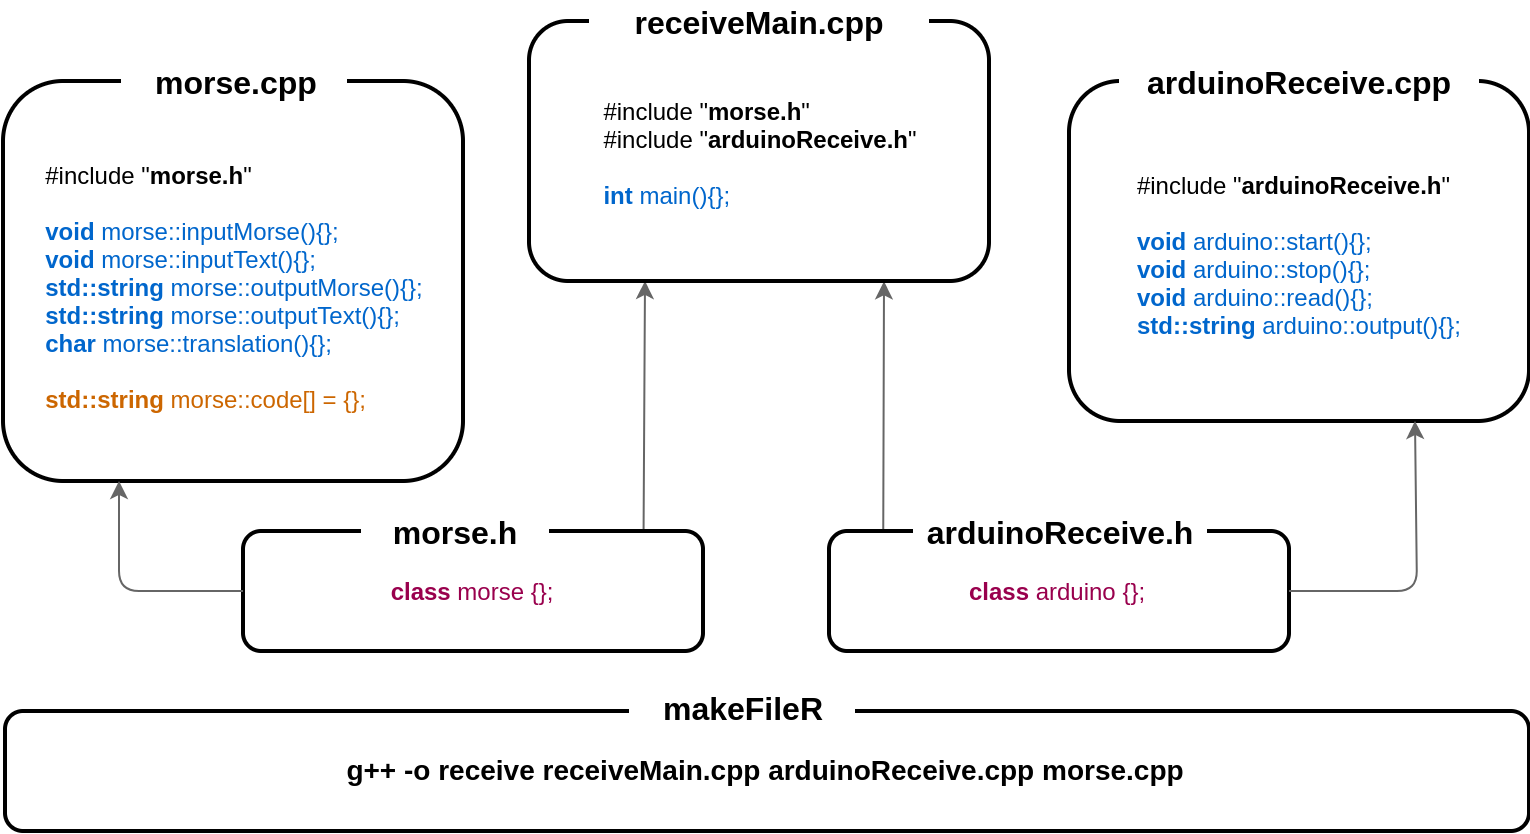
\includegraphics[width=15cm]{rCodeStructure}
\caption{Code structure for \textbf{receiving} phase.}	
\label{fig:re_code}
\end{figure}


\subsection{Class \texttt{arduino}}

For handling the output received from Arduino we created a class called \verb|arduino|:

\begin{lstlisting}
class arduino
{

	public:
	void start();
	void stop();
	void read();
	void clear();
	std::string output();

	private:
	FILE* arduinoFile;
	std::vector<int> durations;
	
};
\end{lstlisting}

\subsection{Functions and variables}

\verb|arduino::start()| - function that 

\verb|arduino::stop()| - function that 

\verb|arduino::read()| - function that 

\verb|arduino::clear()| - function that 

\verb|arduino::output()| - function that 





\subsection{Main}


\subsection{Fire it up with makefile}

The code is compiled in an analogous way to the \textbf{broadcasting} phase. Once you have all 5 files in one place run from the command line:

\begin{snugshade}
\verb|make -f makeFileR|
\end{snugshade}

A new binary file called \verb|receive| will be produced.

To run the receiving phase type in the command line:

\begin{snugshade}
\verb|./receive|
\end{snugshade}

If this doesn't work, you might need to run the binary as \verb|root|:

\begin{snugshade}
\verb|sudo ./receive|
\end{snugshade}

And the code should be up and running!

\subsection{Test run}

Weather you've already built the \textbf{broadcasting} phase or not, you can run the binary \verb|receive| and see for yourself what the \textit{Objectif Morse} is capable of!

When the code is started you will see the modest:

\begin{snugshade}
\verb|Input time:|
\end{snugshade}

You should type the time in seconds during which the setup will "listen" to the incomming message.

If you have a flashlight at hand you may want to play a little with broadcasting Morse signals by hand. Just type for example 30 seconds and hit Enter:

\begin{snugshade}
\begin{verbatim}
Input time:
30
\end{verbatim}
\end{snugshade}


\section{How does it work}





\subsection{Arduino connection}

The picture below describes how to build the electronic circuit for the \textbf{receiving} phase. It consists of a phototransistor and a 10 000$\Omega$ resistor. \textbf{Always double-check the circuit that gets connected to Arduino} because the mistakes may sometimes be sad for your little Italian device. It's a good habit to first upload the code to Arduino (only connecting it to a USB A-B cable) then disconnect the Arduino from the USB and assemble the circuit in a powered-off mode.

We use the analog pin A0, as well as the 5V pin to serve as our (+) and the GND pin to serve as (-).

\begin{figure}[H]
\centering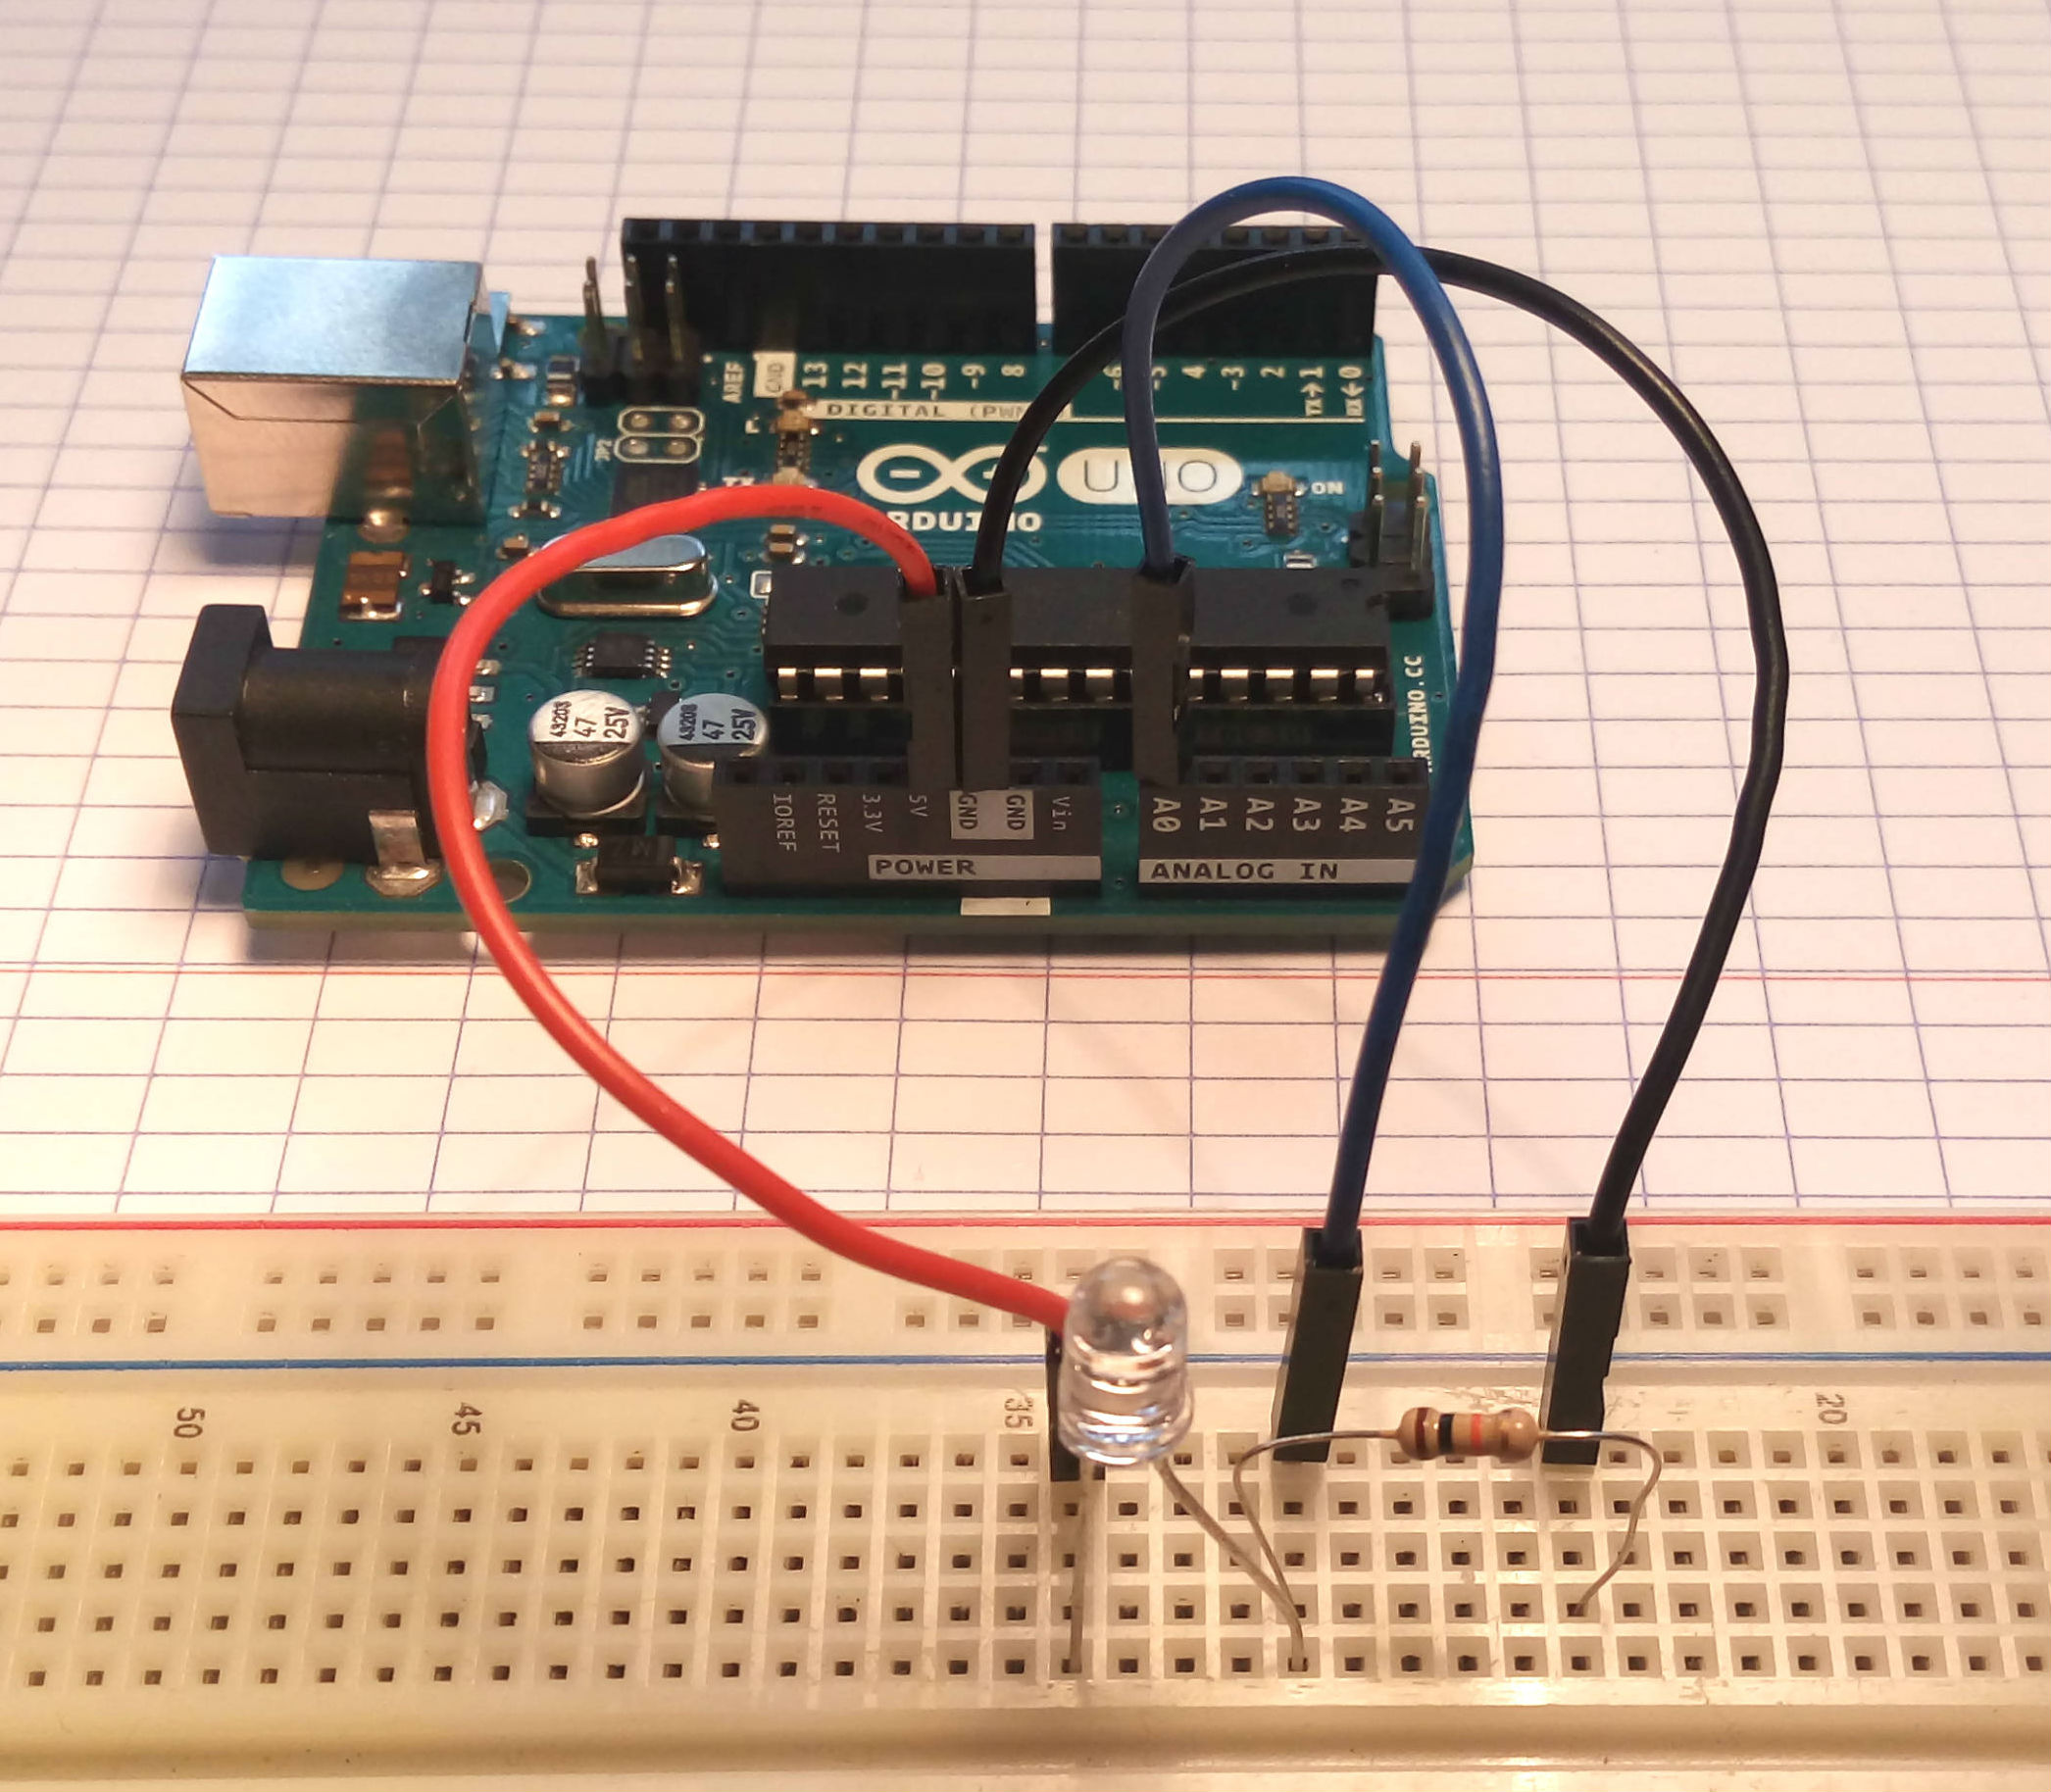
\includegraphics[width=8cm]{receive_circuit}
\caption{Electronic circuit for the receiving phase.}				
\label{fig:receiving_circuit}
\end{figure}




\subsection{Arduino code}

In this part we describe the contents of the Arduino code \verb|arduinoCode.ino|. This code is written in C language and should be uploaded to your Arduino device. We recommend downloading Arduino IDE for Linux - a neat little program in which you can easily verify and upload Arduino codes. It also comes with a library of examples that could be useful in your future projects.

\subsubsection{Arduino's job}

The aim of the Arduino code is to identify the signal as Low (\verb|L|) or High (\verb|H|) and to measure the time duration in \textit{ms} of that state.

One of the sample Arduino outputs can be:

\begin{snugshade}
\begin{verbatim}
L 200
H 200
L 600
\end{verbatim}
\end{snugshade}

Which has the interpretation as follows: Low state lasted 200 \textit{ms}, then High state lasted 200 \textit{ms}, then Low state lasted 600 \textit{ms}, and so on...




\subsubsection{Variables}

Variables used in the code:

\verb|analogInPin| - specifies the analog pin that we connect to, in our case it's A0.

\verb|sensorValue| - the value of voltage read using \verb|analogRead()| function. This value describes the luminosity as seen directly by the phototransistor. It's a number between 0 and 1023.

\verb|sensorMean| - the mean luminosity, assuming that the LED diode is not lit up. It is calculated in the calibration part of the code.

\verb|sensorThres| - the lower threshold of the High state. Any value higher then this will be considered as a High state. It is calculated in the calibration part of the code.

\verb|prevSignal| - a boolean describing the state from which the change has just occured. It is \verb|true| when the previous state was High and \verb|false| when the previous state was Low.

\verb|timeDuration| - the total time of the last Low or High state.

\verb|timePrev| - the time in \textit{ms} at which the change from Low to High or from High to Low occured, measured from the beginning of the program operation.

In the graph below we present in a closer detail how the Low and High state is interpreted by the Arduino code. Anything that is higher then \verb|sensorThres| is interpreted as a High state. Anything that is 10 from \verb|sensorMean| (either way) is interpreted as a Low state. There are two gaps, where the signal is not interpreted as either High or Low, which probably should be thought over...

\begin{figure}[H]
\centering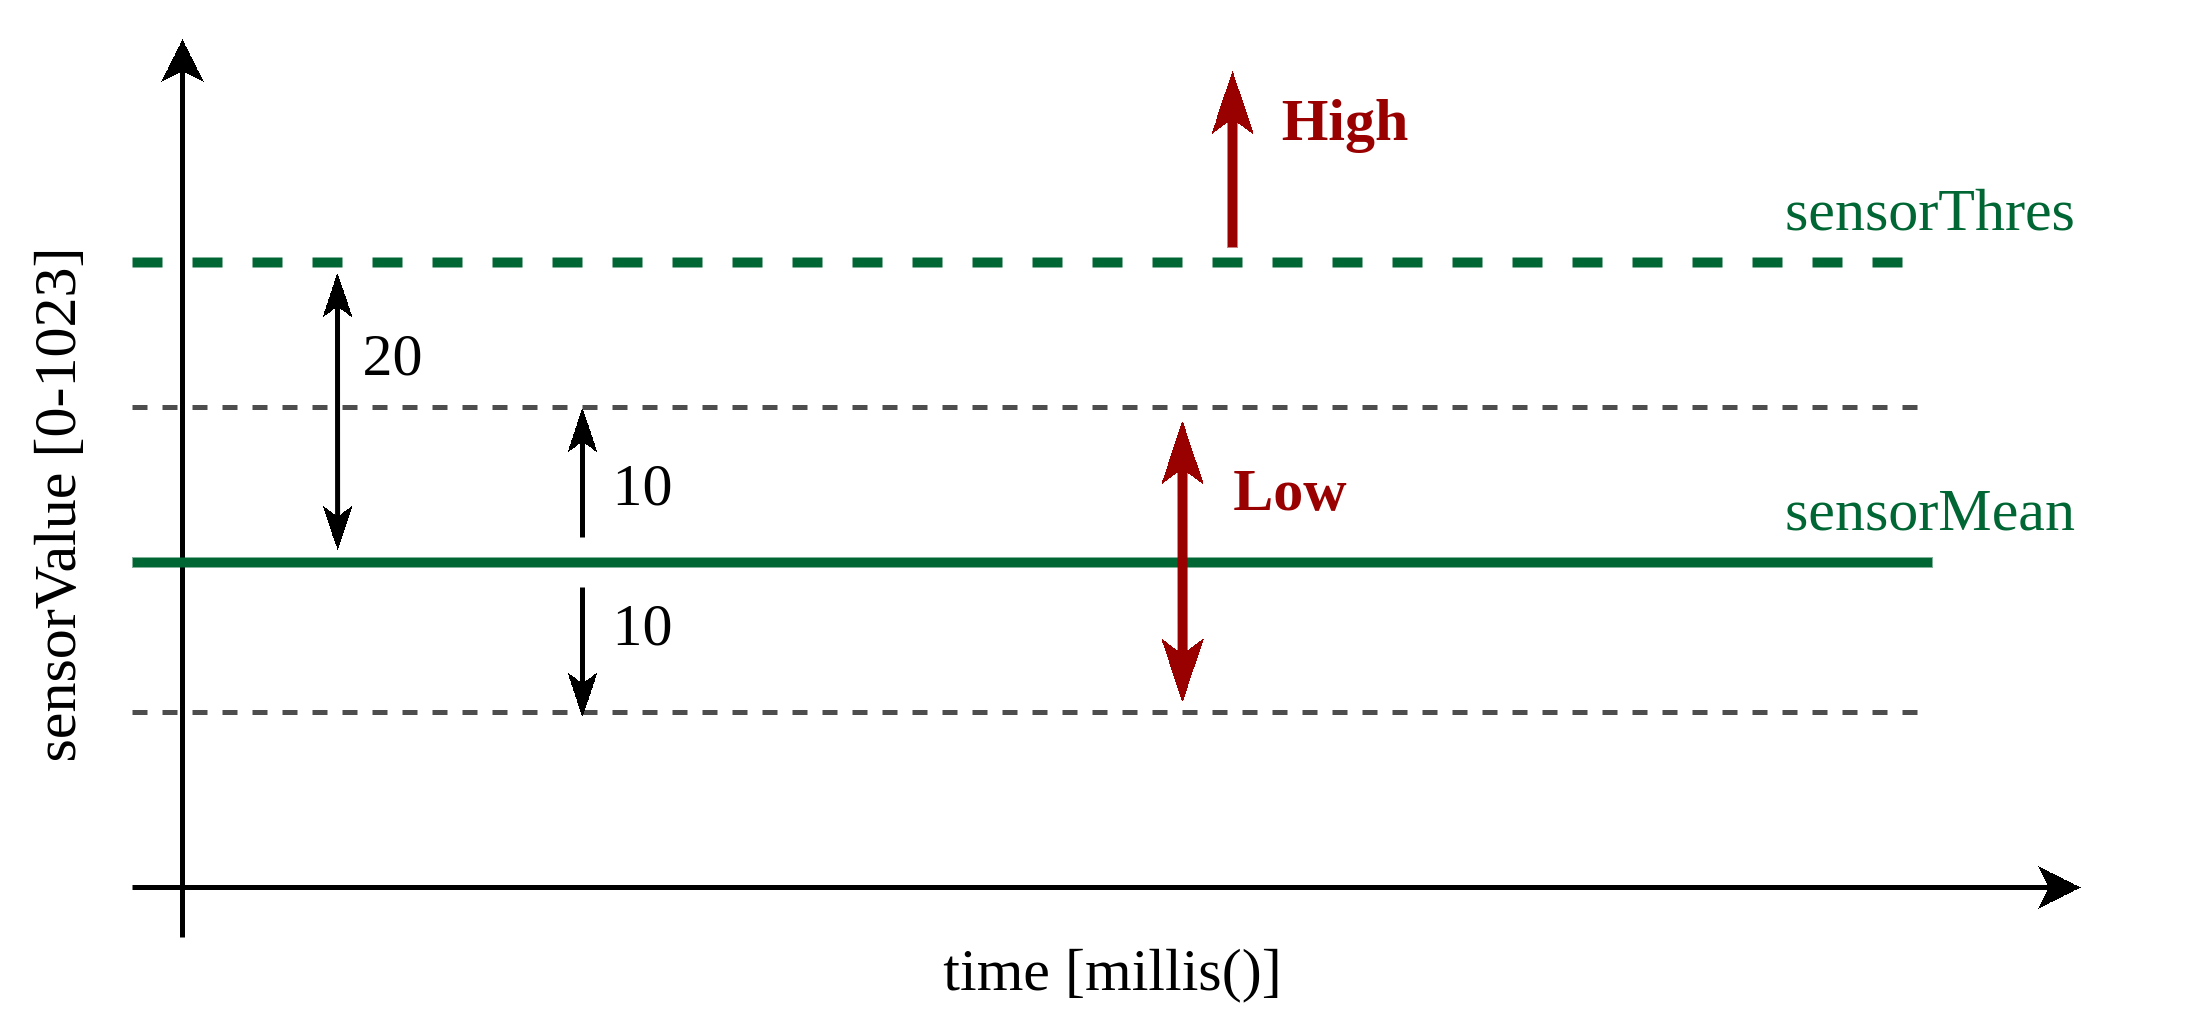
\includegraphics[scale=0.18]{arduinocode}
\caption{Interpretation of Low and High states using defined variables.}				
\label{fig:arduino_code}
\end{figure}



\subsubsection{Calibration}

The aim of the calibration is to measure the mean luminosity around the phototransistor and to use this information for further processing of the luminosity that comes from the LED diode itself. This mean luminosity will be present everytime we have a Low state in our signal - interpreted as "darkness".

The need to do this comes from the fact that we can send our coded messages during sunny or gloomy day or during the night, and we want the Arduino to correctly interpret what part of the luminosity comes from the general brightness of the surroundings and what part are the changes due to the LED diode.

The aim of the calibration is to obtain the value \verb|sensorMean|. This is performed by reading 10 values of \verb|sensorValue| in 100 \textit{ms} time steps and calculating their arithmetic average.

\subsubsection{Identifying the voltage changes}

Inside the \verb|loop()| function, the \verb|sensorValue| is read at the beginning and then if certain conditions are met, we have either signal changing from Low to High or changing from High to Low.

The signal is changing from Low to High when the voltage read is greater than the \verb|sensorThres| and when the previous signal was Low (when the \verb|prevSignal| is set to false). This condition is comprised in the following \verb|if()| statement:

\begin{lstlisting}
if (sensorValue > sensorThres && !prevSignal)
\end{lstlisting}

\begin{figure}[H]
\centering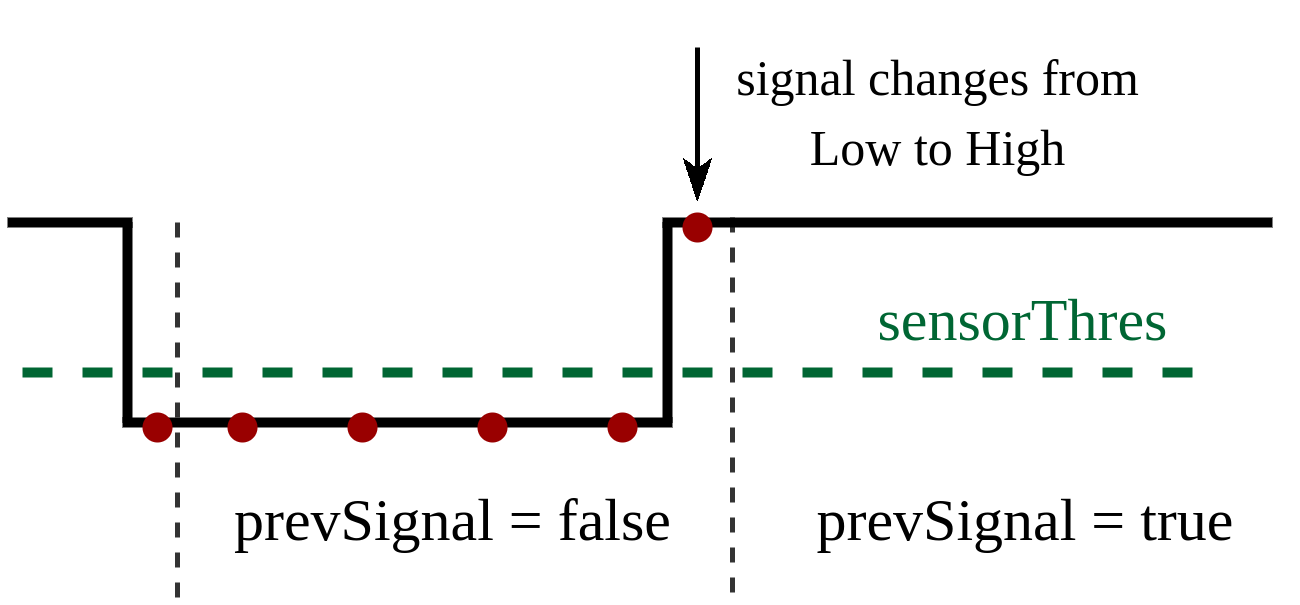
\includegraphics[scale=0.18]{lowtohigh}
\caption{Signal changing from Low to High. Red dots represent the \texttt{sensorValue} measurement.}				
\label{fig:arduino_code}
\end{figure}

The signal is changing from High to Low when the voltage read is within 10 from the \verb|sensorMean| value and when the previous signal was High (when the \verb|prevSignal| is set to true). This condition is comprised in the following \verb|if()| statement:

\begin{lstlisting}
if (sensorValue - sensorMean < 10 && prevSignal)
\end{lstlisting}

\begin{figure}[H]
\centering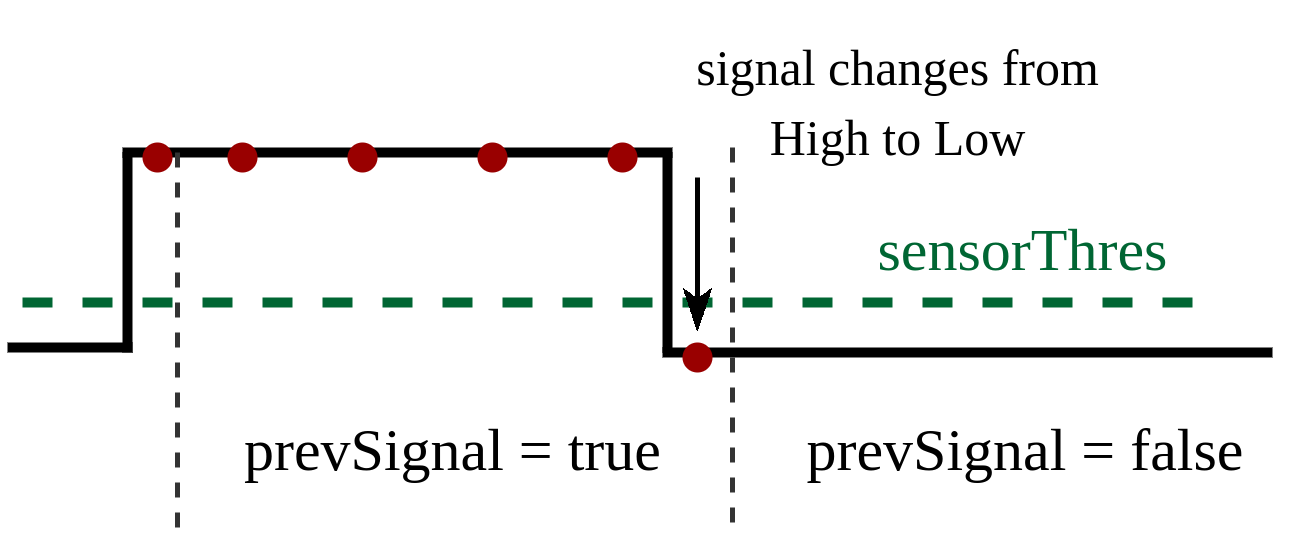
\includegraphics[scale=0.18]{hightolow}
\caption{Signal changing from High to Low.}				
\label{fig:arduino_code}
\end{figure}

\subsubsection{Measuring the time durations}

Each time we enter one of the two \verb|if()| statements, the time of the last finished state (High or Low) must be identified, measured and printed on the Serial Monitor.

Additionally, a flag \verb|prevSignal| is always changed to describe the currently entered state.

For the purpose of measuring the time durations we use the built-in Arduino function \verb|millis()|. This function measures the time in \textit{ms} that has passed from the beginning of the operation of the program. It can therefore be viewed as an absolute time. It increases while the Arduino operates and is only set back to zero, when the Arduino is reset.

The variable \verb|timeDuration|, which we are interested in, is therefore measured as a difference between the current absolute time and the time at which the last change occured. Looking at the Fig. [\ref{fig:timedur}], the red dot represents the first voltage measurement made after the signal has changed from High to Low. The time of the last High state has to be measured and it is equal to \verb|millis() - timePrev|, where the 
\textcolor{cadr}{\texttt{timePrev}} in this case is the time at which the High state has begun.


\begin{figure}[H]
\centering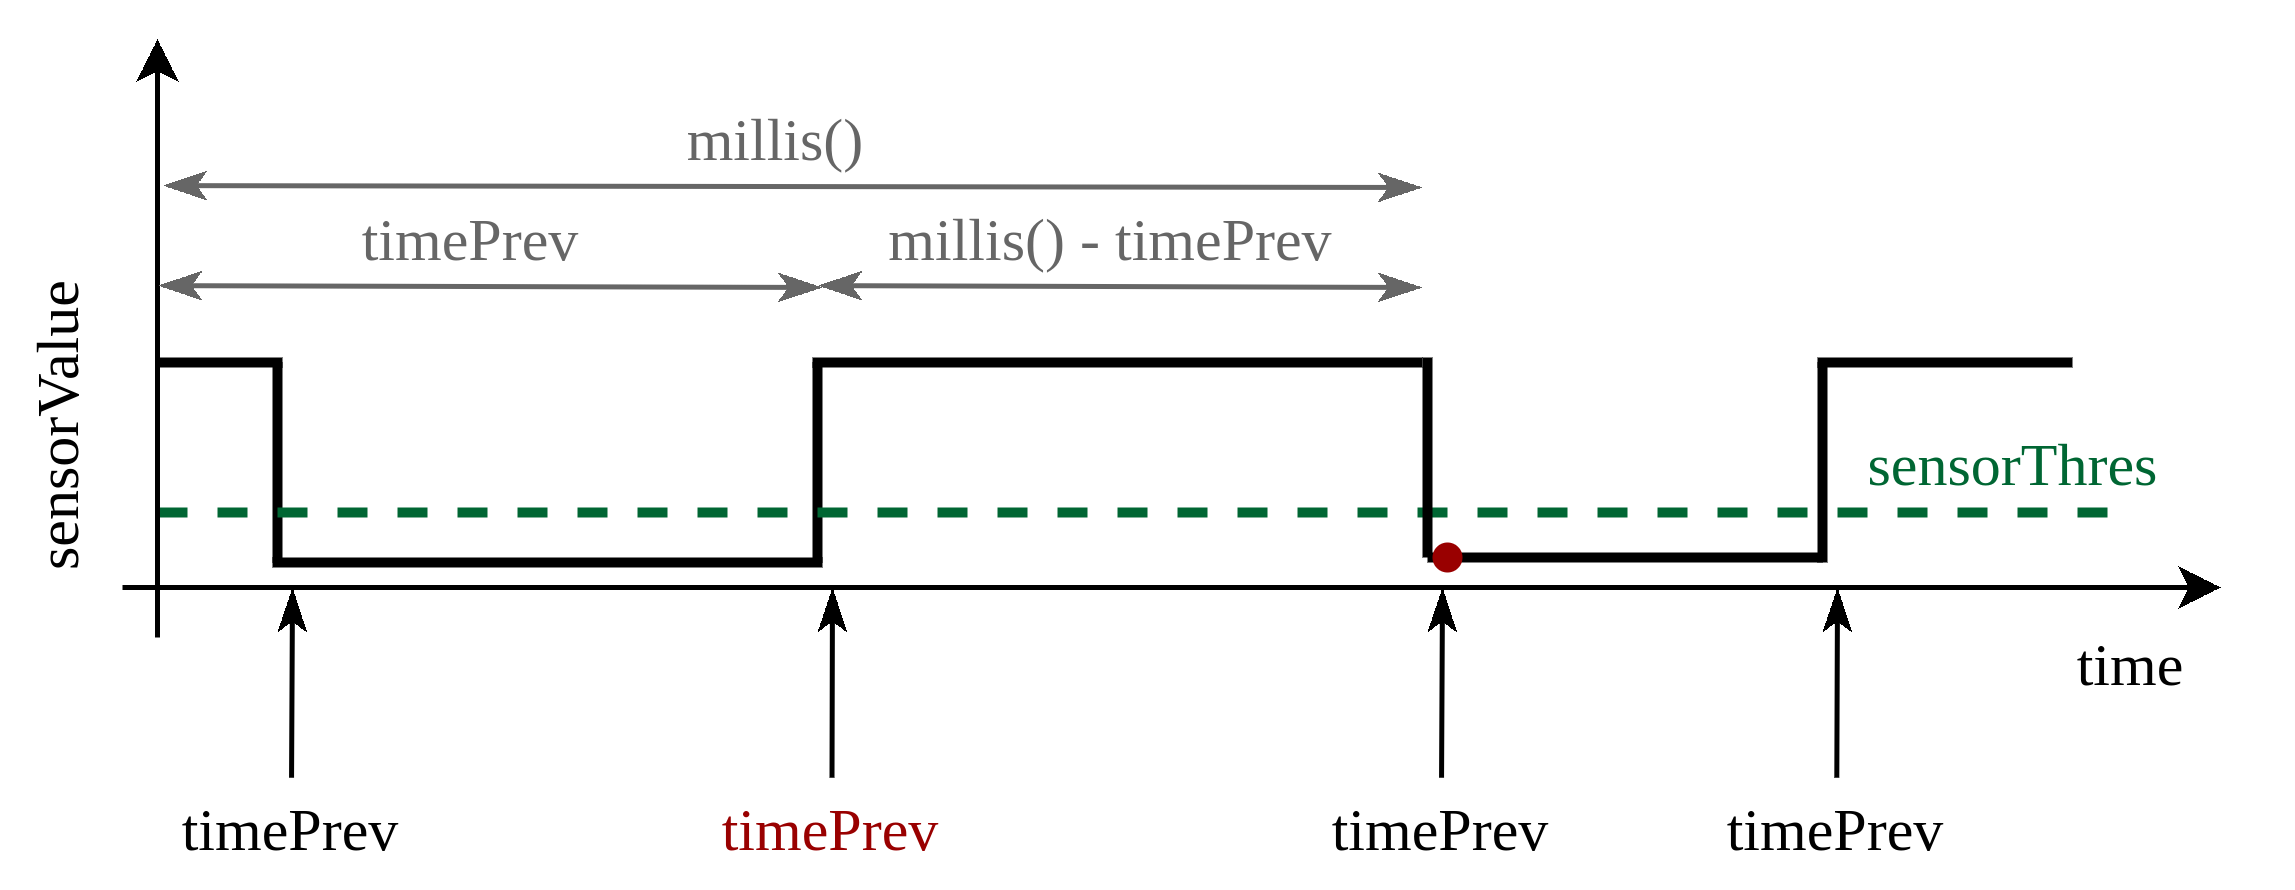
\includegraphics[scale=0.18]{timedurations}
\caption{Measuring the time durations.}				
\label{fig:timedur}
\end{figure}

The identification of the last finished state as High or Low is made by entering the correct \verb|if()| condition, and then accordingly we print on the Serial Monitor either \verb|"H"| or \verb|"L"|, followed by the current value of the variable \verb|timeDuration|.

The corresponding flag needs to be raised. If we entered the High state, the \verb|prevSignal| has to be set to true and if we entered the Low state, the \verb|prevSignal| has to be set to false.

Finally, it should be noted that entering the \verb|if()| conditions happen only at changes between Low and High states. Outside of this changes, the \verb|loop()| function simply keeps measuring the \verb|sensorValue|.

\chapter{Putting it all together}


\begin{figure}[H]
\centering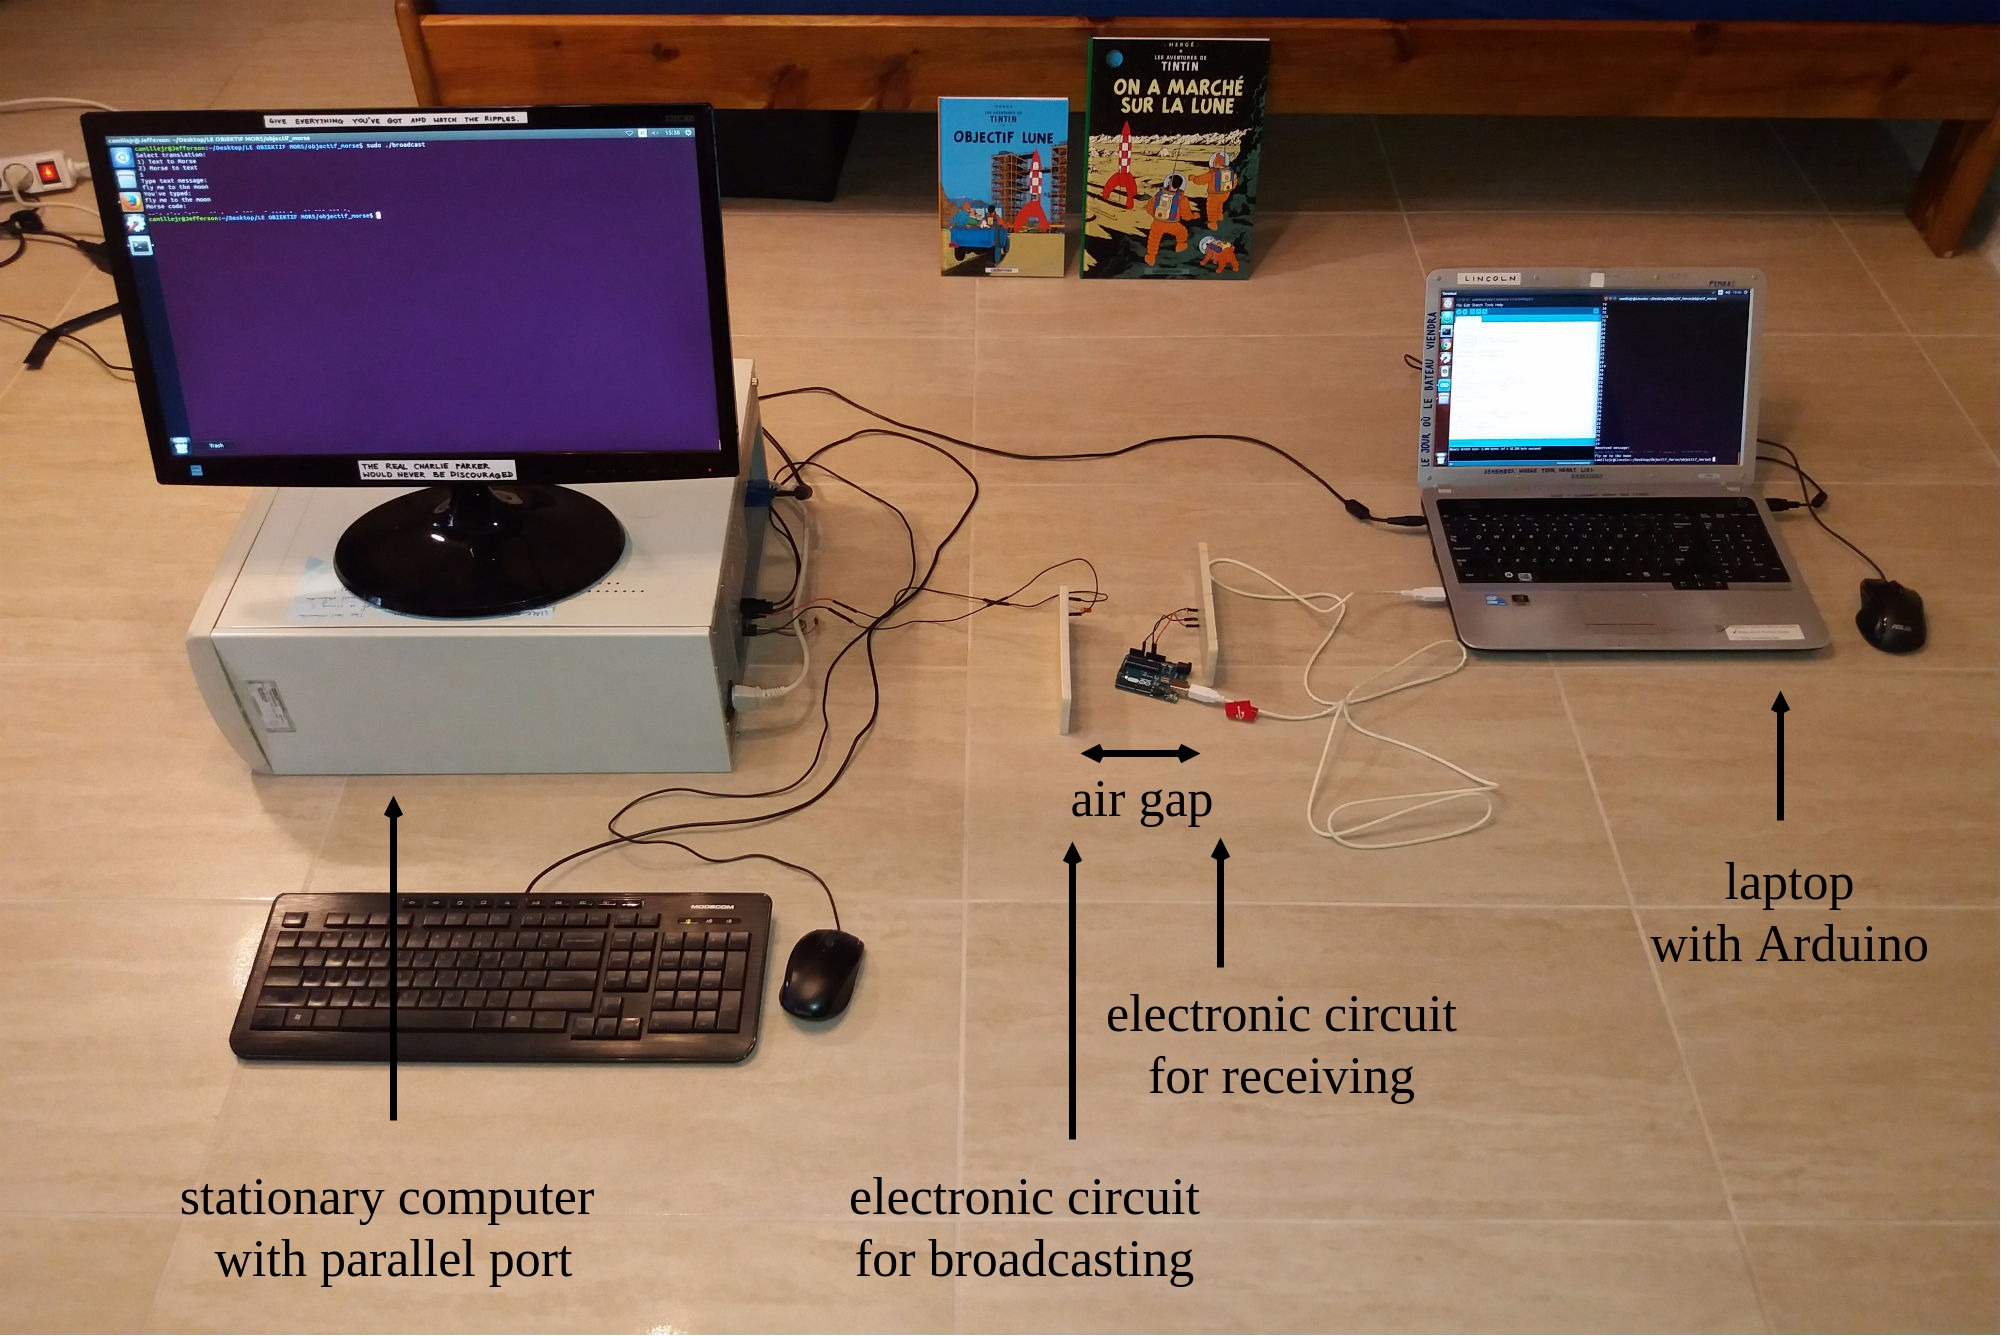
\includegraphics[width=15cm]{full_setup}
\caption{Objectif Morse full setup.}				
\label{fig:full_setup}
\end{figure}

\begin{figure}[H]
\centering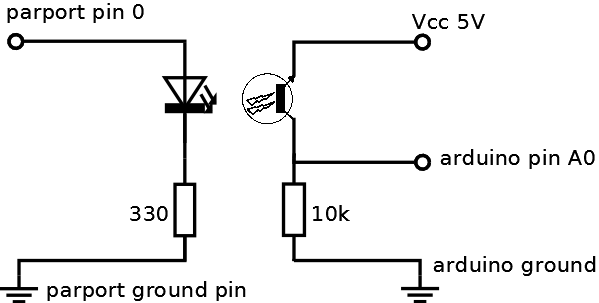
\includegraphics[width=8cm]{scheme}
\caption{Scheme of the electronic circuits put together.}				
\label{fig:circuits}
\end{figure}

\begin{figure}[H]
\centering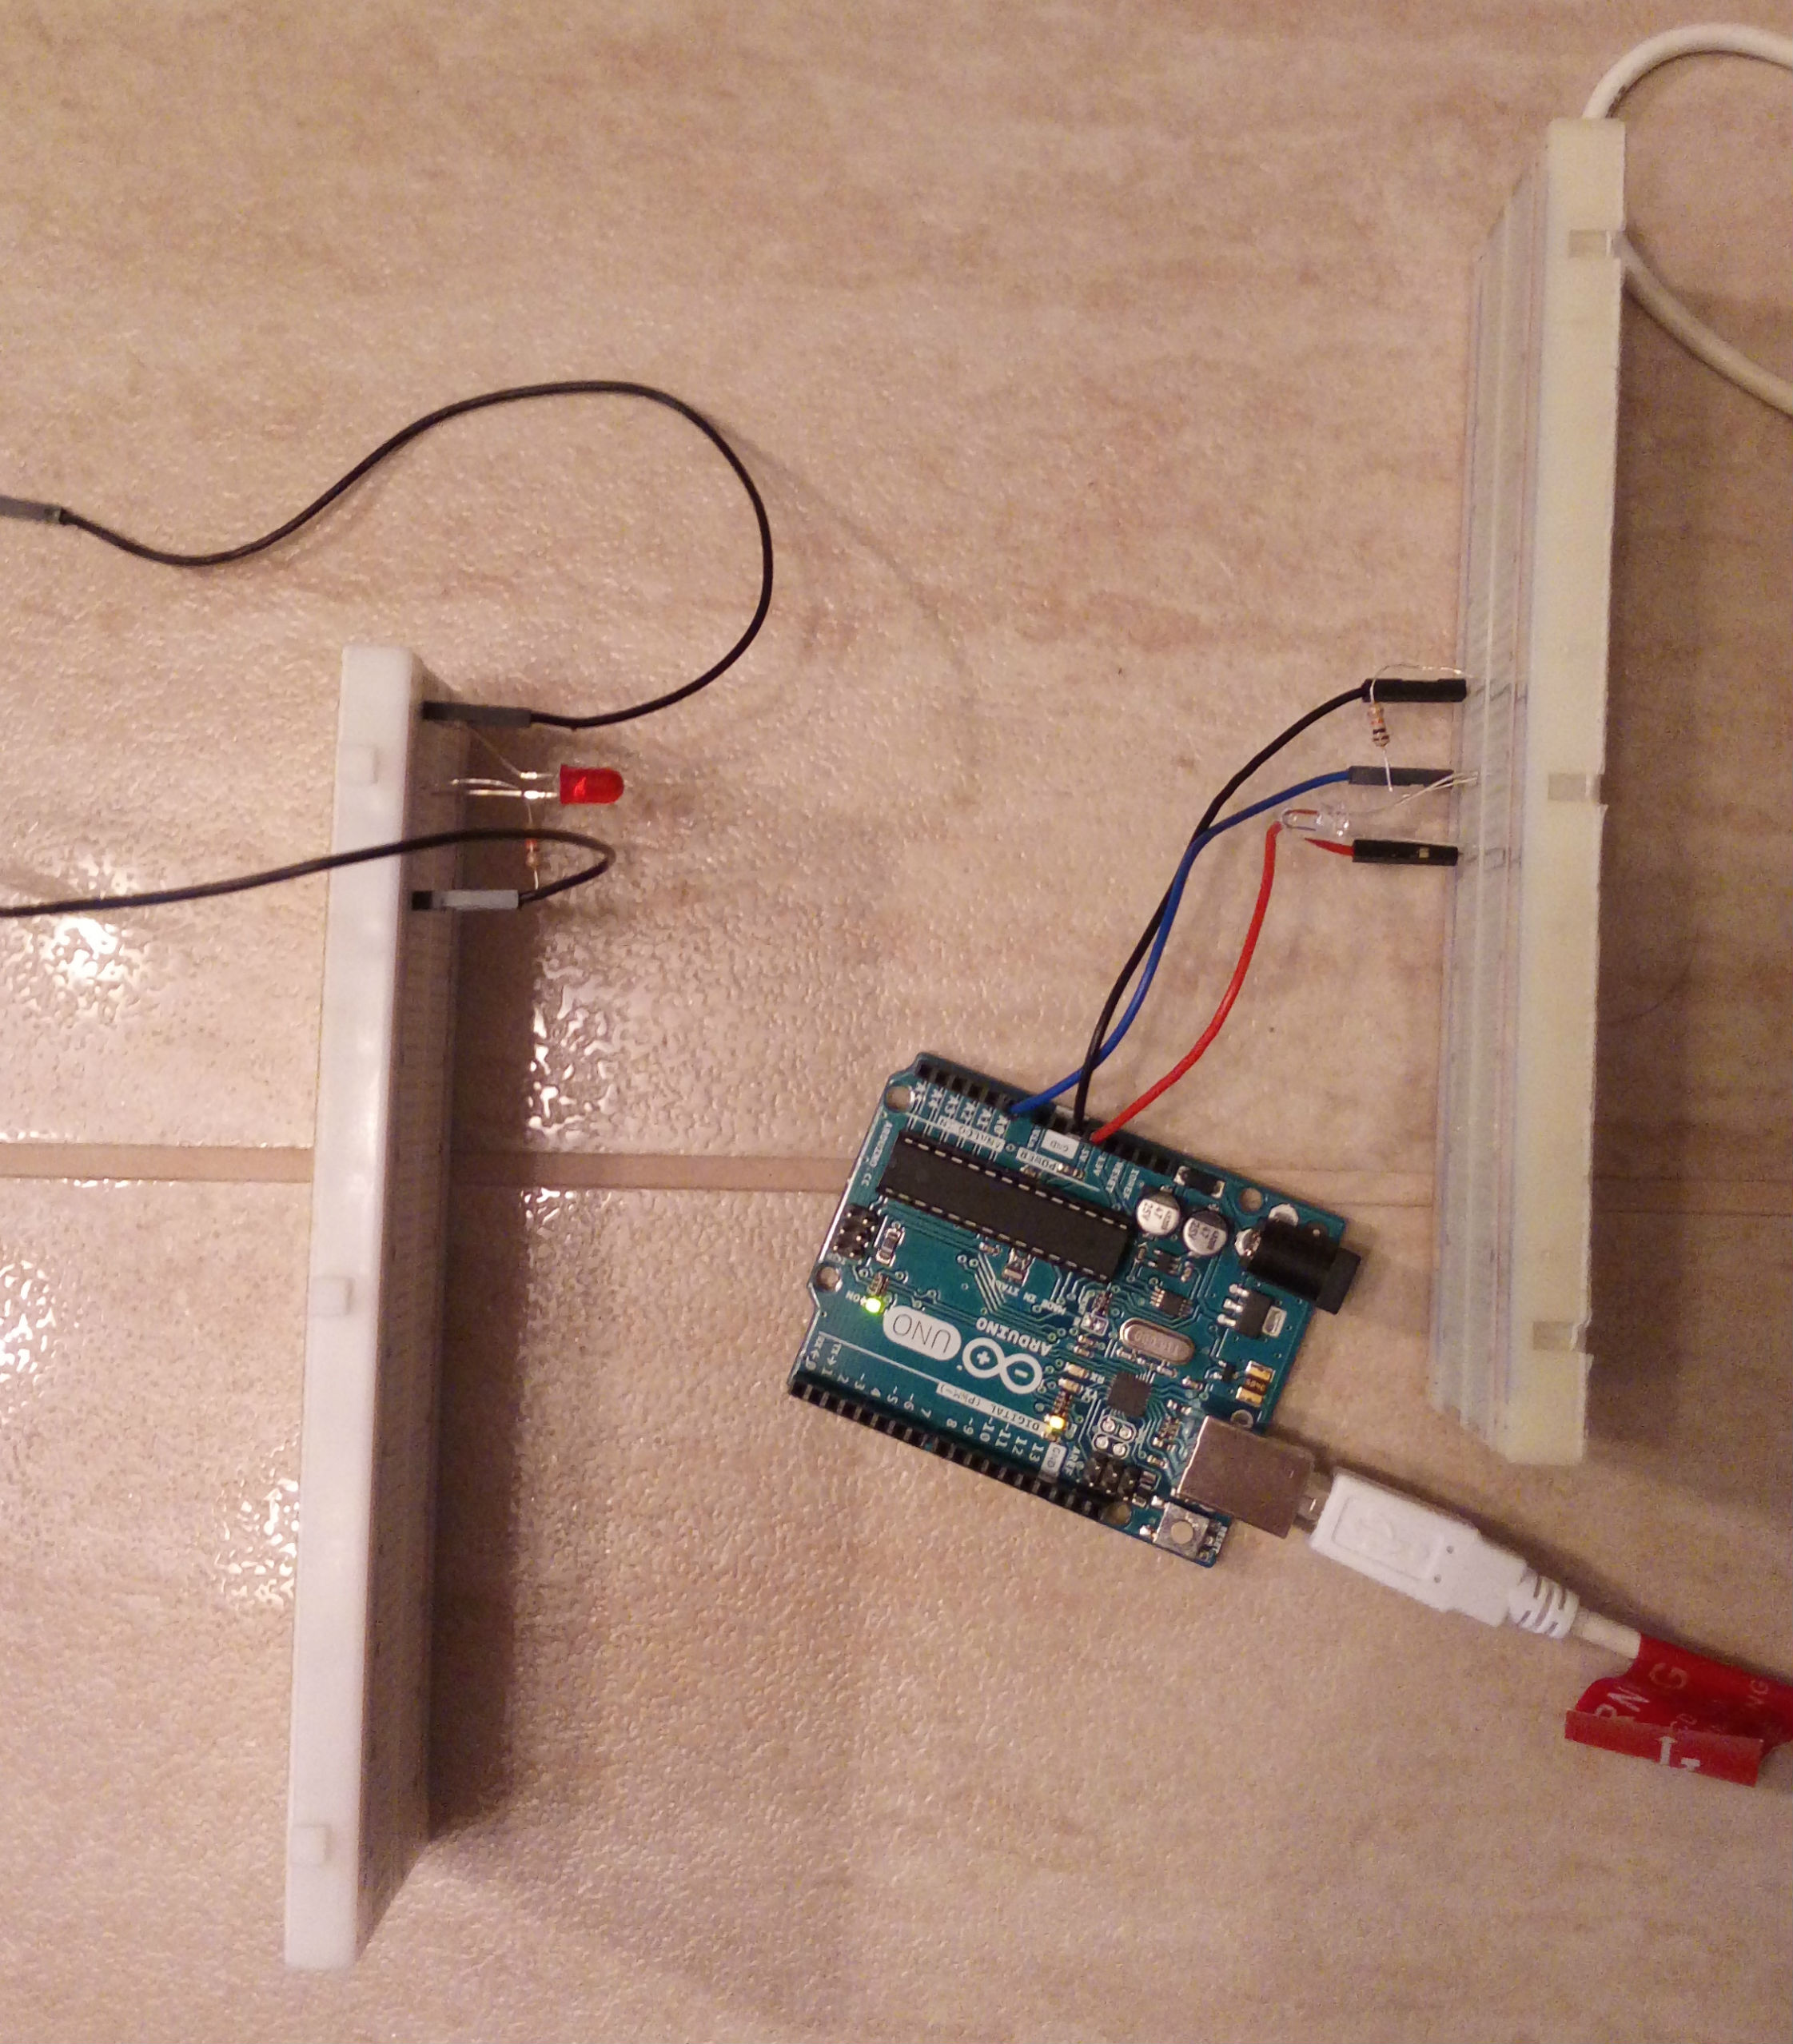
\includegraphics[width=8cm]{circuits}
\caption{Electronic circuits put together.}				
\label{fig:circuits_pic}
\end{figure}



\chapter{It doesn't end here}

This last chapter is a collection of post-credit scenes where we present a few of our ways of exploiting the machinery that we have created.

\section{Reading secret alien messages}

Now it's your time to have some more fun! Forget about the \textbf{broadcasting} part, take the flashlight and try to create the message yourself by shining on the phototransistor. Hopefully you'll do better then me, it took me about 20 unsuccessful trials before I broadcasted the first letter of my name. Good luck.


\section{How far can it go?}

~ 22cm separation was the maximum that we've observed during daylight of a gloomy day, with closed window shades and with no artificial light in the room.


\section{How fast can it go?}

The parameter \verb|dotTime| alows you to control the speed of the transmission. Feel free to play around with it! We've observed that \verb|dotTime < 2000 ms| is when the transmission errors begin to occur. It is also dependent on the distance between LED diode and the phototransistor and on the general luminosity.


\section{Sending a picture}

How uneffective it would be to transfer images between computers using Morse? Let's find out!

\section{Light to sound}

At some point we realized that it won't be a lot of effort to replace light Morse transmission with sound Morse transmission! Using a microphone and a buzzer you can achieve pretty much the same thing.

\section{Want to see more?}

There was a lot of more ideas and unfortunately not always enough free time.

One day we would like to extend the project to transmit messages over larger distances. Perhaps use a laser beam and a solar panel? Could this be a new way of the internet-free communication between neighbours? Although quite susceptible to the man-in-the-middle attack... But what if neighbours used an optical fiber hidden in the ground?...

As Cliff Stoll once said \cite{cliff_stoll}: 

\textit{I'm interested in seeing where the curiosity will lead to, not: oh, where have we been.}

We encourage you to explore, learn, make a lot of mistakes and the most important: have a lot of pleasure of finding things out. Perhaps we'll hear from you soon when you share with us your ideas!

\newpage

\begin{thebibliography}{50}

\bibitem{objectif_lune} \hyperlink{https://fr.wikipedia.org/wiki/Objectif_Lune}{\textit{Les Aventures De Tintin: Objectif Lune}}, Hergé

\bibitem{le_lotus_bleu} \hyperlink{https://fr.wikipedia.org/wiki/Le_Lotus_bleu}{\textit{Les Aventures De Tintin: Le Lotus Bleu}}, Hergé

\bibitem{ioperm} \hyperlink{http://man7.org/linux/man-pages/man2/ioperm.2.html}{\texttt{ioperm}}, Linux Programmer's Manual

\bibitem{cliff_stoll} \hyperlink{https://www.youtube.com/watch?v=xHEIOgONq6A}{Cliff Stoll: Good Science}

\end{thebibliography}

\end{document}
